\chapter{Electronics}
\label{p:em:el12}

%\nts{Status: Ready for evaulation.  Dynamic references need adding where previous chapters are referred to.}

\section{Introduction}
Electronics and electrical devices surround us in daily life. From the street lights and water pumps to computers and digital phones, electronics have enabled the digital revolution to occur. All electronics are built on a backbone of simple circuits, and so an understanding of circuits is vital in understanding more complex devices.

This chapter will explain the basic physics principles of many of the components of electronic devices.  We will begin with an explanation of capacitors and inductors. We see how these are used in tuning a radio.  Next, we look at {\bf active} components such as transistors and operational amplifiers. Lastly, the chapter will finish with an explanation of digital electronics, including logic gates and counting circuits. 

Before studying this chapter, you will want to remind yourself of:
\begin{itemize}
%\item The meaning of voltage ($V$), current ($I$) and resistance ($R$), as covered in Grade 10 (see chapter~\ref{p:ElecCircuitsG10}), and Grade 11 (see chapter~\ref{p:em:ec11}).
\item The meaning of voltage ($V$), current ($I$) and resistance ($R$), as covered in Grade 10, and Grade 11.
\item Capacitors in electric circuits, as covered in Grade 11 (see section 17.6).
\item Semiconductors, as covered in Grade 11 (see chapter 20).
\item The meaning of an alternating current (see section 28.3).
\item Capacitance ($C$) and Inductance ($L$) (see section 28.4).
\end{itemize}
%\nts{Dynamic references need to be put in place to direct the reader to the other chapters.}

\section{Capacitive and Inductive Circuits}
%\begin{syllabus}
%\item The learner must be able to Perform calculations on capacitive circuits using the formula:	$V^2  =  I^2(R^2 + X_C^2)$
%\item The learner must be able to Understand that in a circuit containing both resistive and reactive components, the ratio $\frac{V}{I}$ is neither pure resistance nor pure reactance.  The ratio is called impedance, $Z$, where $Z  = \sqrt{R^2+X_C^2}$ and is measured in $\Omega$ s.
%\item The learner must be able to Understand that any coil has inductance, but also resistance.  So a coil can be considered as a resistance and an inductance in series.  The impedance of an inductor is given by: $Z  = \sqrt{R^2+X_L^2}$
%\end{syllabus}

Earlier in Grade 12, you were shown alternating currents (AC) and you saw that the voltage and the current varied with time.  If the AC supply is connected to a resistor, then the current and voltage will be proportional to each other.  This means that the current and voltage will `peak' at the same time.  We say that the current and voltage are {\bf in phase}.  This is shown in Figure~\ref{fig:VIres}.

\begin{figure}[htbp]
\begin{center}
\begin{pspicture}(0,-2.5)(10,3)
\psline[arrows=->](0,0)(9,0)
\uput[r](8.5,-0.5){Time}
\psplot[xunit=0.0111,%
		plotstyle=curve]%
		{0}{720}{x sin}
\psplot[xunit=0.0111,%
		plotstyle=curve,%
		linestyle=dashed]%
		{0}{720}{x sin 2 mul}
\uput[r](1.1,2){Current}
\uput[r](1.1,1){Voltage}
\end{pspicture}
\caption{The voltage and current are in phase when a resistor is connected to an alternating voltage.}
\label{fig:VIres}
\end{center}
\end{figure}

When a capacitor is connected to an alternating voltage, the maximum voltage is proportional to the maximum current, but the maximum voltage does not occur at the same time as the maximum current.  The current has its maximum (it peaks) one quarter of a cycle before the voltage peaks.  Engineers say that the `current leads the voltage by $90^{\circ}$'.  This is shown in Figure~\ref{fig:VIcap}.

\begin{figure}[htbp]
\begin{center}
\begin{pspicture}(0,-2.5)(10,3)
\psline[arrows=->](0,0)(9,0)
\uput[r](8.5,-0.5){Time}
\psplot[xunit=0.0111,%
		plotstyle=curve]%
		{0}{720}{x sin}
\psplot[xunit=0.0111,%
		plotstyle=curve,%
		linestyle=dashed]%
		{0}{720}{x 90 add sin 2 mul}
\uput[r](0.1,2){Current}
\uput[r](1.1,1){Voltage}
\end{pspicture}
\caption{The current peaks (has its maximum) one quarter of a wave before the voltage when a capacitor is connected to an alternating voltage.}
\label{fig:VIcap}
\end{center}
\end{figure}

For a circuit with a capacitor, the instantaneous value of $\frac{V}{I}$ is not constant.  However, the value of $\frac{V_{\mathrm{max}}}{I_{\mathrm{max}}}$ is useful, and is called the {\bf capacitive reactance} ($X_{C}$) of the component.  Because it is still a voltage divided by a current (like resistance), its unit is the ohm.  The value of $X_{C}$ ($C$ standing for capacitor) depends on its capacitance ($C$) and the frequency ($f$) of the alternating current (in South Africa 50 Hz).

\equ{X_{C} = \frac{V_{\mathrm{max}}}{I_{\mathrm{max}}} = \frac{1}{2 \pi f C}}{eq:xc}

Inductors are very similar, but the current peaks $90^{\circ}$ after the voltage.  This is shown in Figure~\ref{fig:VIind}.  Engineers say that the `current lags the voltage'.  Again, the ratio of maximum voltage to maximum current is called the reactance --- this time inductive reactance ($X_{L}$).  The value of the reactance depends on its inductance ($L$).

\equ{X_{L} = \frac{V_{\mathrm{max}}}{I_{\mathrm{max}}} = 2 \pi f L}{eq:xl}

\begin{figure}[htbp]
\begin{center}
\begin{pspicture}(0,-2)(10,3)
\psline[arrows=->](0,0)(9,0)
\uput[r](8.5,-0.5){Time}
\psplot[xunit=0.0111,%
		plotstyle=curve]%
		{0}{720}{x sin}
\psplot[xunit=0.0111,%
		plotstyle=curve,%
		linestyle=dashed]%
		{0}{720}{x 90 sub sin 2 mul}
\uput[r](2.1,2){Current}
\uput[r](1.1,1){Voltage}
\end{pspicture}
\caption{The current peaks (has its maximum) one quarter of a wave after the voltage when an inductor is connected to an alternating voltage.}
\label{fig:VIind}
\end{center}
\end{figure}

\Definition{Reactance}{The ratio of the maximum voltage to the maximum current when a capacitor or inductor is connected to an alternating voltage.  The unit of reactance is the ohm.}

While inductive and capacitive reactances are similar, in one sense they are opposites.  For an inductor, the current peaks $90^{\circ}$ {\bf after} the voltage.  For a capacitor the current peaks $90^{\circ}$ {\bf ahead} of the voltage.  When we work out the total reactance for an inductor and a capacitor in series, we use the formula
\equ{X_{\mathrm{total}} = X_{L} - X_{C}}{eq:xtotal}

to take this into account.  This formula can also be used when there is more than one inductor or more than one capacitor in the circuit.  The total reactance is the sum of all of the inductive reactances minus the sum of all the capacitive reactances.  The magnitude (number) in the final result gives the ratio of maximum voltage to maximum current in the circuit as a whole.  The sign of the final result tells you its phase.  If it is positive, the current peaks $90^{\circ}$ after the voltage, if it is negative, the current peaks $90^{\circ}$ before the voltage.


If a series circuit contains resistors as well, then the situation is more complicated.  The maximum current is still proportional to the maximum voltage, but the phase difference between them won't be $90^{\circ}$.  The ratio between the maximum voltage and maximum current is called the {\bf impedance} ($Z$), and its unit is also the ohm.  Impedances are calculated using this formula:
\equ{Z = \sqrt{X^{2} + R^{2}}}{eq:z}

where $X$ is the total reactance of the inductors and capacitors in the circuit, and $R$ is the total resistance of the resistors in the circuit.


It is easier to understand this formula by thinking of a right angled triangle.  Resistances are drawn horizontally, reactances are drawn vertically.  The hypotenuse of the triangle gives the impedance.  This is shown in Figure~\ref{fig:XRZtriangle}.

\begin{figure}[htbp]
\begin{center}
\begin{pspicture}(-0.5,-1)(9,6)
\psline[arrows=->](0,0)(4,0)
\psline[arrows=->](4,0)(4,5)
\psline[doubleline=true, doublesep=0.05, arrows=->](0,0)(4,5)
\uput[r](1.5,-0.5){Resistance $R$}
\uput[r](4.3,2.5){Reactance $X$}
\uput[r](-0.3,3.0){Impedance $Z$}
\end{pspicture}
\caption{Visualizing the relationship between reactance, resistance and impedance.}
\label{fig:XRZtriangle}
\end{center}
\end{figure}

\Definition{Impedance}{The maximum voltage divided by the maximum current for any circuit. The unit of impedance is the ohm.}

It is important to remember that when resistors and inductances (or capacitors) are in a circuit, the current will not be in phase with the voltage, so the impedance is not  a resistance.  Similarly the current won't be exactly $90^{\circ}$ out of phase with the voltage so the impedance isn't a reactance either.

The following simulation allows you to build some circuits with capacitors and inductors.
Phet simulation on circuit building: SIYAVULA-SIMULATION:http://cnx.org/content/m39523/latest/#id63458
\begin{wex}{The impedance of a coil}{Calculate the maximum current in a coil in a South African motor which has a resistance of 5 $\Omega$ and an inductance of 3 mH.  The maximum voltage across the coil is 6 V.  You can assume that the resistance and inductance are in series.}{\begin{enumerate} \item Calculate the reactance of the coil $X_{L} = 2 \pi f L = 2 \pi \times 50 \times 0,003 = 0,942 \; \Omega$ 
\item Calculate the impedance of the coil $Z = \sqrt{X^{2} + R^{2}} = \sqrt{ 0,942^{2} + 5^{2}} = 5,09 \; \Omega$\
\item Calculate the maximum current $I_{\mathrm{max}} = V_{\mathrm{max}} / Z = 6 / 5,09 = 1,18$ A. \end{enumerate}}
\end{wex}

\begin{wex}{An RC circuit}{Part of a radio contains a 30 $\Omega$ resistor in series with a 3 $\mu$F capacitor.  What is its impedance at a frequency of 1 kHz?}{\begin{enumerate} \item 
Calculate the reactance of the capacitor

\nequ{X_{C} = \frac{1}{2 \pi f C} = \frac{1}{2 \pi \times 10^{3} \times 3 \times 10^{-6}} = 53,05 \; \Omega}
\item Calculate the impedance $Z = \sqrt{X^{2} + R^{2}} = \sqrt{ 53,05^{2} + 30^{2}} = 60,9 \; \Omega$  \end{enumerate}}
\end{wex}

\Exercise{Capacitive and Inductive Circuits}{
\begin{enumerate}
\item Why is the instantaneous value of $\frac{V}{I}$ of little use in an AC circuit containing an inductor or capacitor?
\item How is the reactance of an inductor different to the reactance of a capacitor?
\item Why can the ratio of the maximum voltage to the maximum current in a circuit with a resistor and an inductor not be called a reactance?
\item An engineer can describe a motor as equivalent to a 30 $\Omega$ resistor in series with a 30 mH inductor.  If the maximum value of the supply voltage is 350 V, what is the maximum current?  Assume that the frequency is 50 Hz.
\item A timer circuit in a factory contains a 200 $\mu$F capacitor in series with a 10 k$\Omega$ resistor.  What is its impedance?  Assume that the frequency is 50 Hz.
\item A 3 mH inductor is connected in series with a 100 $\mu$F capacitor.  The reactance of the combination is zero.  What is the frequency of the alternating current?
\end{enumerate}}

\begin{IFact}{Most factories containing heavy duty electrical equipment (e.g. large motors) have to pay extra money to their electricity supply company because the inductance of the motor coils causes the current and voltage to get out of phase.  As this makes the electricity distribution network less efficient, a financial penalty is incurred.  The factory engineer can prevent this by connecting capacitors into the circuit to reduce the reactance to zero, as in the last question above.  The current and voltage are then in phase again.  We can't calculate the capacitance needed in this chapter, because the capacitors are usually connected in parallel, and we have only covered the reactances and impedances of series circuits.} \end{IFact}

\section{Filters and Signal Tuning}
%\begin{syllabus}
%\item The learner must be able to Describe how capacitors and inductors can be used as filters for currents of certain frequencies
%\item The learner must be able to For a circuit containing both an inductor and a capacitor (LRC circuit), calculate the impedance using the expression $Z  = \sqrt{R^2+(X_L-X_C)^2}$
%\item The learner must be able to State the relationship between the phase of the voltages across an inductor, a resistor and a capacitor in an LRC circuit.
%\item The learner must be able to Explain what is meant by resonance and calculate the resonant frequency of an LRC circuit
%\item The learner must be able to Explain how LRC circuits are used for signal tuning and calculate values of relevant quantities needed to receive specific frequencies
%\end{syllabus}

\subsection{Capacitors and Inductors as Filters}
We have already seen how capacitors and inductors pass current more easily at certain frequencies than others. To recap: if we examine the equation for the reactance of a capacitor, we see that the frequency is in the denominator. Therefore, when the frequency is low, the capacitive reactance is very high. This is why a capacitor blocks the flow of DC and low frequency AC because its reactance increases with decreasing frequency. 


When the frequency is high, the capacitive reactance is low. This is why a capacitor allows the flow of high frequency AC because its reactance decreases with increasing frequency.


Therefore putting a capacitor in a circuit blocks the low frequencies and allows the high frequencies to pass.  This is called a high pass filter.  A filter like this can be used in the `treble' setting of a sound mixer or music player which controls the amount of high frequency signal reaching the speaker.  The more high frequency signal there is, the `tinnier' the sound.  A simple high pass filter circuit is shown in Figure~\ref{fig:hipass}.

\begin{figure}[H]
\begin{center}
\begin{pspicture}(0,0)(7,5)
\psline(0,4)(5,4)
\psline(5.3,4)(7,4)
\psline(5,3.5)(5,4.5)
\psline(5.3,3.5)(5.3,4.5)
\psline(0,0)(7,0)
\psline(2,0)(2,1)
\psline(2,3)(2,4)
\psarc(2,1.25){0.25}{-90}{90}
\psarc(2,1.75){0.25}{-90}{90}
\psarc(2,2.25){0.25}{-90}{90}
\psarc(2,2.75){0.25}{-90}{90}
\uput[r](5.5,4.5){$C$}
\uput[r](6.5,4.5){next part of circuit...}
\uput[r](2.5,2){$L$}
\end{pspicture}
\caption{A high pass filter.  High frequencies easily pass through the capacitor and into the next part of the circuit, while low frequencies pass through the inductor straight to ground.}
\label{fig:hipass}
\end{center}
\end{figure}

Similarly, if we examine the equation for the reactance of an inductor, we see that inductive reactance increases with increasing frequency. Therefore, when the frequency is low, the inductive reactance is very low. This is why an inductor allows the flow of DC and low frequency AC because its reactance decreases with decreasing frequency. 


When the frequency is high, the inductive reactance is high. This is why an inductor blocks the flow of high frequency AC because its reactance increases with increasing frequency.


Therefore putting an inductor in a circuit blocks the high frequencies and allows the low frequencies to pass.  This is called a low pass filter.  A filter like this can be used in the `bass' setting of a sound mixer or music player which controls the amount of low frequency signal reaching the speaker.  The more low frequency signal there is, the more the sound `booms'.  A simple low pass filter circuit is shown in Figure~\ref{fig:lopass}.


\begin{figure}[H]
\begin{center}
\begin{pspicture}(0,0)(7,4)
\psline(0,2.5)(4,2.5)
\psline(6,2.5)(7,2.5)
\psline(1.5,1)(2.5,1)
\psline(1.5,1.3)(2.5,1.3)
\psline(0,0)(7,0)
\psline(2,0)(2,1)
\psline(2,1.3)(2,2.5)
\psarc(4.25,2.5){0.25}{0}{180}
\psarc(4.75,2.5){0.25}{0}{180}
\psarc(5.25,2.5){0.25}{0}{180}
\psarc(5.75,2.5){0.25}{0}{180}
\uput[r](2.3,1.7){$C$}
\uput[r](5,3.1){$L$}
\uput[r](6.5,3.1){next part of circuit...}
\end{pspicture}
\caption{A low pass filter.  Low frequencies pass through the inductor and into the next part of the circuit, while high frequencies pass through the capacitor straight to ground.}
\label{fig:lopass}
\end{center}
\end{figure}
 
\subsection{LRC Circuits, Resonance and Signal Tuning}
A circuit containing a resistor, a capacitor and an inductor all in series is called an LRC circuit.  Because the components are in series, the current through each component at a particular time will be the same as the current through the others.  The voltage across the resistor will be in phase with the current.  The voltage across the inductor will be $90^{\circ}$ ahead of the current (the current always follows or lags the voltage in an inductor).  The voltage across the capacitor will be $90^{\circ}$ behind the current (the current leads the voltage for a capacitor).  The phases of the voltages for the inductor and capacitor relative to the common current are shown in Figure~\ref{fig:VLCR}.

\begin{figure}[H]
\begin{center}
\begin{pspicture}(0,-2)(10,3)
\psline[arrows=->](0,0)(9,0)
\uput[r](8.8,0.2){Time}
\psplot[xunit=0.0111,%
		plotstyle=curve]%
		{0}{720}{x sin}
\uput[r](1.3,1){$I$}
\psplot[xunit=0.0111,%
		plotstyle=curve,%
		linestyle=dashed]%
		{0}{720}{x 90 add sin 1.5 mul}
\uput[r](0.1,1.5){$V_{L}$}
\psplot[xunit=0.0111,%
		plotstyle=curve,%
		linestyle=dotted]%
		{0}{720}{x 90 sub sin 2.0 mul}
\uput[r](2.1,2.0){$V_{C}$}
\end{pspicture}
\caption{The voltages across the separate components of an LRC circuit. Looking at the peaks, you see that the voltage across the inductor $V_{L}$ `peaks' first, followed $90^{\circ}$ later by the current $I$, followed $90^{\circ}$ later by the voltage across the capacitor $V_{C}$.  The voltage across the resistor is not shown --- it is in phase with the current and peaks at the same time as the current.}
\label{fig:VLCR}
\end{center}
\end{figure}


The reactance of the inductor is $2 \pi f L$, and the reactance of the capacitor is $1 / 2 \pi f C$ but with the opposite phase.  So the total reactance of the LRC circuit is 
\nequ{X = X_{L} - X_{C} = 2 \pi f L - \frac{1}{2 \pi f C}}
The impedance of the circuit as a whole is given by
\nequ{Z = \sqrt{X^{2} + R^{2}} = \sqrt{\left( 2 \pi f L - \frac{1}{2 \pi f C} \right)^{2} + R^{2}}}
At different frequencies, the impedance will take different values.  The impedance will have its smallest value when the positive inductive reactance cancels out the negative capacitive reactance.  This occurs when
\nequ{2 \pi f L = \frac{1}{2 \pi f C}}
so the frequency of minimum impedance must be
\nequ{f = \frac{1}{2 \pi \sqrt{LC}}}
This is called the {\bf resonant frequency} of the circuit.  This is the frequency at which you can get the largest current for a particular supply voltage.  It is also called the {\bf natural frequency} of the circuit.  This means the frequency at which the circuit would oscillate by itself.

\Definition{Resonance}{Resonance occurs when a circuit is connected to an alternating voltage at its natural frequency. A very large current can build up in the circuit, even with minimal power input.}

An LRC circuit is very useful when we have a signal containing many different frequencies, and we only want one of them.  If a mixed signal like this is connected to an LRC circuit, then only the resonant frequency (and other frequencies close to it) will drive measureable currents.  This means that an LRC circuit can select one frequency from a range.  This process is called {\bf signal tuning}.

\begin{IFact}{When you set up a radio antenna, and amplify the radio signal it receives, you find many different bands of frequencies --- one from each radio station.  When you listen to the radio, you only want to listen to one station.  An LRC circuit in the radio (the tuning circuit) is set so that its resonant frequency is the frequency of the station you want to listen to.  This means that of the many radio stations broadcasting, you only hear one.  When you adjust the tuning dial on the radio, it changes the capacitance of the capacitor in the tuning circuit.  This changes the resonant frequency, and this changes the radio station that you will hear.}\end{IFact}

\Exercise{Filters and Signal Tuning}{
\begin{enumerate}
\item Which component would you use if you wanted to block low frequencies?
\item Which component would you use if you wanted to block high frequencies?
\item Calculate the impedance of a series circuit containing a 50 $\Omega$ resistor, a 30 $\mu$F capacitor and a 3 mH inductor for frequencies of (a) 50 Hz, (b) 500 Hz, and (c) 5 000 Hz.
\item Calculate the resonant frequency of the circuit in the previous question, part (c).
\item A radio station broadcasts at a frequency of 150 kHz.  The tuning circuit in the radio contains a 0.3 mH inductor.  What is the capacitance of the capacitor needed in the tuning circuit if you want to listen to this radio station?
\item State the relationship between the phase of the voltages across an inductor, a resistor and a capacitor in an LRC circuit.
\item Explain what is meant by resonance.
\item Explain how LRC circuits are used for signal tuning, for example in a radio.
\end{enumerate}}

\section{Active Circuit Elements}

The components you have been learning about so far --- resistors, capacitors and inductors --- are called {\bf passive} components.  They do not change their behaviour or physics and therefore always have the same response to changes in voltage or current.  {\bf Active} components are quite different.  Their response to changes in input allows them to make amplifiers, calculators and computers.

\subsection{The Diode}
%\begin{syllabus}
%\item The learner must be able to Describe a diode as a device used in electronics that allows current to flow in one direction only.
%\item The learner must be able to Explain that a diode consists of two doped semi-conductors joined together so that the resistance is low when connected one way and very high the other way. 
%\end{syllabus}

A diode is an electronic device that allows current to flow in one direction only. 

\begin{figure}[H]
\begin{center}
\begin{pspicture}(-1,0)(3,2)
%\psgrid
\diode(0,1)(2,1){}
\pcline[offset=-0.4cm]{->}(0,1)(2,1)
\bput{:U}{direction of current}
\rput(0.6,1.2){$+$}
\rput(1.4,1.2){$-$}
\end{pspicture}
\caption{Diode circuit symbol and direction of flow of current.}
\end{center}
\end{figure}

A diode consists of two doped semi-conductors joined together so that the resistance is low when connected one way and very high the other way. 

\begin{figure}[H]
\begin{center}
\begin{pspicture}(-1,0)(9,3.4)
%\psgrid
\pnode(0,0){A}
\pnode(0,3){B}
\pnode(3,3){C}
\pnode(3,0){D}
\battery(B)(A){}
\uput[r](0.2,2){$+$}
\uput[r](0.2,1){$-$}
\diode(B)(C){}
\lamp(C)(D){}
\psline(D)(A)
\pnode(5,0){E}
\pnode(5,3){F}
\pnode(8,3){G}
\pnode(8,0){H}
\battery(E)(F){}
\uput[r](5.2,1){$+$}
\uput[r](5.2,2){$-$}
\diode(F)(G){}
\lamp(G)(H){}
\psline(H)(E)
\end{pspicture}
\caption{Operation of a diode. (Left) The diode is forward biased and current is permitted. The negative terminal of the battery is connected to the negative terminal of the diode. (Right) The diode is reverse biased and current flow is not allowed. The negative terminal of the battery is connected to the positive terminal of the diode.}
\end{center}
\end{figure}

A full explanation of diode operation is complex.  Here is a simplified description.  The diode consists of two semiconductor blocks attached together.  Neither block is made of pure silicon --- they are both {\bf doped}.  Doping was described in more detail in Section 10.3. 
%\nts{A proper, dynamic reference needs to be given here}  

In short, p-type semiconductor has fewer free electrons than normal semiconductor.  `P' stands for `positive', meaning a lack of electrons, although the material is actually neutral.  The locations where electrons are missing are called {\bf holes}.  This material can conduct electricity well, because electrons can move into the holes, making a new hole somewhere else in the material.  Any extra electrons introduced into this region by the circuit will fill some or all of the holes.  

In n-type semiconductor, the situation is reversed.  The material has more free electrons than normal semiconductor.  `N' stands for `negative', meaning an excess of electrons, although the material is actually neutral.

When a p-type semiconductor is attached to an n-type semiconductor, some of the free electrons in the n-type move across to the p-type semiconductor.  They fill the available holes near the junction.  This means that the region of the n-type semiconductor nearest the junction has no free electrons (they've moved across to fill the holes).  This makes this n-type semiconductor positively charged.  It used to be electrically neutral, but has since lost electrons.

The region of p-type semiconductor nearest the junction now has no holes (they've been filled in by the migrating electrons).   This makes the p-type semiconductor negatively charged.  It used to be electrically neutral, but has since gained electrons.  

Without free electrons or holes, the central region can not conduct electricity well.  It has a high resistance, and is called the {\bf depletion band}.  This is shown in Figure~\ref{fig:deplayer}.  

\begin{figure}[H]
\begin{center}
\begin{pspicture}(1,1)(6,3.6)
%\psgrid[gridcolor=gray,subgriddiv=10]
\psframe[fillstyle=solid,fillcolor=lightgray](1,1)(3,3)
\psframe[fillstyle=solid,fillcolor=white](3,1)(4,3)
\psframe[fillstyle=solid,fillcolor=gray](4,1)(6,3)
\multirput(1,1)(0.2,0){10}{\multirput(0,0)(0,0.2){10}{\psdot[dotstyle=o](0.1,0.1)}}
\multirput(4,1)(0.2,0){10}{\multirput(0,0)(0,0.2){10}{\psdot(0.1,0.1)}}
\uput[u](2,3){p-type}
\uput[u](5,3){n-type}
\pcline[linestyle=none](3.5,1)(3.5,3)
\lput{:U}{\footnotesize{depletion band}}
\bput{:U}{}
\end{pspicture}
\caption{A diode consists of two doped semi-conductors joined together so that the resistance is low when connected one way and very high the other way.}
\label{fig:deplayer}
\end{center}
\end{figure}

You can explain the high resistance in a different way.  A free electron in the n-type semiconductor will be repelled from the p-type semiconductor because of its negative charge.  The electron will not go into the depletion band, and certainly won't cross the band to the p-type semiconductor.  You may ask, ``But won't a free electron in the p-type semiconductor be attracted across the band, carrying a current?''  But there are no free electrons in p-type semiconductor, so no current of this kind can flow.

If the diode is reverse-biased, the $+$ terminal of the battery is connected to the n-type semiconductor.  This makes it even more negatively charged.  It also removes even more of the free electrons near the depletion band.  At the same time, the $-$ terminal of the battery is connected to the p-type silicon.  This will supply free electrons and fill in more of the holes next to the depletion band.  Both processes cause the depletion band to get wider.  The resistance of the diode (which was already high) increases.  This is why a reverse-biased diode does not conduct.

Another explanation for the increased resistance is that the battery has made the p-type semiconductor {\it more negative} than it used to be, making it repel any electrons from the n-type semiconductor which attempt to cross the depletion band.

On the other hand, if the diode is forward biased, the depletion band is made narrower.  The negative charge on the p-type silicon is cancelled out by the battery.  The greater the voltage used, the narrower the depletion band becomes.  Eventually, when the voltage is about 0,6 V (for silicon) the depletion band disappears.  Once this has occurred, the diode conducts very well.  



\Exercise{The Diode}{
\begin{enumerate}
\item What is a diode?
\item What is a diode made of?
\item What is the term which means that a diode is connected the `wrong way' and little current is flowing?
\item Why is a diode able to conduct electricity in one direction much more easily than the other?
\end{enumerate}}

\subsection{The Light-Emitting Diode (LED)}
%\begin{syllabus}
%\item The learner must be able to Describe the LED as a diode that emits light when conducting.
%\item The learner must be able to Give examples of the use LEDs in everyday life
%\end{syllabus}

A light-emitting diode (LED) is a diode device that emits light when charge flows in the correct direction through it. If you apply a voltage to force current to flow in the direction the LED allows, it will light up.

\begin{figure}[H]
\begin{center}
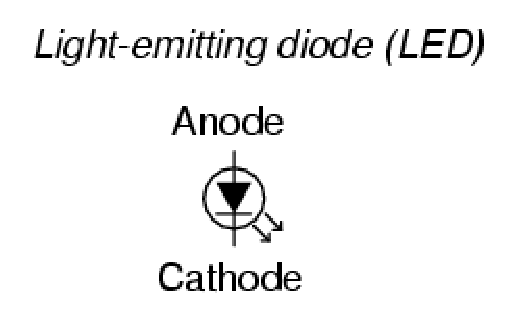
\includegraphics[scale=0.5]{../../epsimages/ledsym.eps}
\caption{Symbol for a light-emitting diode with anode and cathode labeled.}
\end{center}
\end{figure}

\Extension{Circuit Symbols}{This notation of having two small arrows pointing away from the device is common to the schematic symbols of all light-emitting semiconductor devices. Conversely, if a device is light-activated (meaning that incoming light stimulates it), then the symbol will have two small arrows pointing toward it. It is interesting to note, though, that LEDs are capable of acting as light-sensing devices: they will generate a small voltage when exposed to light, much like a solar cell on a small scale. This property can be gainfully applied in a variety of light-sensing circuits.}

The colour depends on the semiconducting material used to construct the LED, and can be in the near-ultraviolet, visible or infrared part of the electromagnetic spectrum.
 
\begin{IFact}{Nick Holonyak Jr. (1928) of the University of Illinois at Urbana-Champaign developed the first practical visible-spectrum LED in 1962.}
\end{IFact}

\subsubsection{Light emission}
The wavelength of the light emitted, and therefore its colour, depends on the materials forming the p-n junction. A normal diode, typically made of silicon or germanium, emits invisible far-infrared light (so it can't be seen), but the materials used for an LED can emit light corresponding to near-infrared, visible or near-ultraviolet frequencies.

\subsubsection{LED applications}
LEDs have many uses.  Some of these are given here.
\begin{itemize}
\item thin, lightweight message displays, e.g. in public information signs (at airports and railway stations, among other places)
\item status indicators, e.g. on/off lights on professional instruments and consumers audio/video equipment
\item infrared LEDs in remote controls (for TVs, VCRs, etc.)
\item clusters of LEDs are used in traffic signals, replacing ordinary bulbs behind coloured glass
\item car indicator lights and bicycle lighting
\item calculator and measurement instrument displays (seven segment displays), although now mostly replaced by LCDs
\item red or yellow LEDs are used in indicator and [alpha]numeric displays in environments where night vision must be retained: aircraft cockpits, submarine and ship bridges, astronomy observatories, and in the field, e.g. night time animal watching and military field use
\item red or yellow LEDs are also used in photographic darkrooms, for providing lighting which does not lead to unwanted exposure of the film
\item illumination, e.g. flashlights (a.k.a. torches, UK), and backlighting for LCD screens
\item signaling/emergency beacons and strobes
\item movement sensors, e.g. in mechanical and optical computer mice and trackballs
\item in LED printers, e.g. high-end colour printers
\end{itemize}

LEDs offer benefits in terms of maintenance and safety.

\begin{itemize}
\item The typical working lifetime of a device, including the bulb, is ten years, which is much longer than the lifetimes of most other light sources.
\item LEDs fail by dimming over time, rather than the abrupt burn-out of incandescent bulbs.
\item LEDs give off less heat than incandescent light bulbs and are less fragile than fluorescent lamps.
\item Since an individual device is smaller than a centimetre in length, LED-based light sources used for illumination and outdoor signals are built using clusters of tens of devices.
\end{itemize}

Because they are monochromatic, LED lights have great power advantages over white lights where a specific colour is required. Unlike the white lights, the LED does not need a filter that absorbs most of the emitted white light. Coloured fluorescent lights are made, but they are not widely available. LED lights are inherently coloured, and are available in a wide range of colours. One of the most recently introduced colours is the emerald green (bluish green, wavelength of about 500 nm) that meets the legal requirements for traffic signals and navigation lights. 

\begin{IFact}{The largest LED display in the world is 36~m high, at Times Square, New York, U.S.A.}
\end{IFact}

There are applications that specifically require light that does not contain any blue component. Examples are photographic darkroom safe lights, illumination in laboratories where certain photo-sensitive chemicals are used, and situations where dark adaptation (night vision) must be preserved, such as cockpit and bridge illumination, observatories, etc. Yellow LED lights are a good choice to meet these special requirements because the human eye is more sensitive to yellow light.

\Exercise{The Light Emitting Diode}{
\begin{enumerate}
\item{What is an LED?}
\item List 5 applications of LEDs.
\end{enumerate}}

\subsection{Transistor}
The diode is the simplest semiconductor device, made up of a p-type semiconductor and an n-type semiconductor in contact. It can conduct in only one direction, but it cannot control the size of an electric current.  Transistors are more complicated electronic components which can control the size of the electric current flowing through them.  

This enables them to be used in amplifiers.  A small signal from a microphone or a radio antenna can be used to control the transistor.  In response, the transistor will then increase and decrease a much larger current which flows through the speakers.

\begin{IFact}{One of the earliest popular uses of transistors was in cheap and portable radios.  Before that, radios were much more expensive and contained glass valves which were fragile and needed replacing.  In some parts of the world you can still hear people talking about their `transistor' --- they mean their portable radio.}\end{IFact}

You can also use a small current to turn the transistor on and off.  The transistor then controls a more complicated or powerful current through other components.  When a transistor is used in this way it is said to be in {\bf switching} mode as it is acting as a remotely controlled switch.  As we shall see in the final sections of this chapter, switching circuits can be used in a computer to process and store digital information.  A computer would not work without the millions (or billions) of transistors in it.

There are two main types of transistor - bipolar transistors (NPN or PNP), and field effect transistors (FETs).  Both use doped semiconductors, but in different ways.  You are mainly required to know about field effect transistors (FETs), however we have to give a brief description of bipolar transistors so that you see the difference.

\subsubsection{Bipolar Transistors}

Bipolar transistors are made of a doped semiconductor `sandwich'.  In an NPN transistor, a very thin layer of p-type semiconductor is in between two thicker layers of n-type semiconductor.  This is shown in Figure~\ref{fig:NPNtrans}.  Similarly an PNP transistor consists of a very thin n-type layer in between two thicker layers of p-type semiconductor.

\begin{figure}[htbp]
\begin{center}
\begin{pspicture}(0,0)(7,3)

\psframe(2,1)(3,2.5)
\uput[r](2.3,1.6){N}
\psframe(3,1)(3.2,2.5)
\uput[r](2.8,1.6){P}
\psframe(3.2,1)(4.2,2.5)
\uput[r](3.5,1.6){N}

\psline(0,1.5)(2,1.5)
\uput[r](0,1.7){Emitter}
\psline(4.2,1.5)(6,1.5)
\uput[r](4.9,1.7){Collector}
\psline(3.1,1)(3.1,0.2)(4.5,0.2)
\uput[r](3.6,0.4){Base}

\end{pspicture}
\caption{An NPN transistor.  This is a type of bipolar transistor.}
\label{fig:NPNtrans}
\end{center}
\end{figure}

In an NPN transistor a small current of electrons flows from the emitter (E) to the base (B).  Simultaneously, a much larger current of electrons flows from the emitter (E) to the collector (C).  If you lower the number of electrons able to leave the transistor at the base (B), the transistor automatically reduces the number of electrons flowing from emitter (E) to collector (C).  Similarly, if you increase the current of electrons flowing out of the base (B), the transistor automatically also increases the current of electrons flowing from emitter (E) to collector (C).  The transistor is designed so that the current of electrons from emitter to collector ($I_{EC}$) is proportional to the current of electrons from emitter to base ($I_{EB}$).  The constant of proportionality is known as the {\bf current gain} $\beta$.  So $I_{EC} = \beta I_{EB}$.

How does it do it?  The answer comes from our work with diodes.  Electrons arriving at the emitter (n-type semiconductor) will naturally flow through into the central p-type since the base-emitter junction is forward biased.  However if none of these electrons are removed from the base, the electrons flowing into the base from the emitter will fill all of the available `holes'.  Accordingly, a large depletion band will be set up.  This will act as an insulator preventing current flow into the collector as well.  On the other hand, if the base is connected to a positive voltage, a small number of electrons will be removed by the base connection.  This will prevent the `holes' in the base becoming filled up, and no depletion band will form. While some electrons from the emitter leave via the base connection, the bulk of them flow straight on to the collector.  You may wonder how the electrons get from the base into the collector (it seems to be reverse biased).  The answer is complicated, but the important fact is that the p-type layer is extremely thin.  As long as there is no depletion layer, the bulk of the electrons will have no difficulty passing straight from the n-type emitter into the n-type collector.  A more satisfactory answer can be given to a university student once band theory has been explained.

Summing up, in an NPN transistor, a small flow of electrons from emitter (E) to base (B) allows a much larger flow of electrons from emitter (E) to collector (C).  Given that conventional current (flowing from $+$ to $-$) is in the opposite direction to electron flow, we say that a small conventional current from base to emitter allows a large current to flow from collector to emitter.

A PNP transistor works the other way.  A small conventional current from emitter to base allows a much larger conventional current to flow from emitter to collector.  The operation is more complicated to explain since the principal charge carrier in a PNP transistor is not the electron but the `hole'.

The operation of NPN and PNP transistors (in terms of conventional currents) is summarized in Figure~\ref{fig:transcur}.

\begin{figure}
\begin{center}
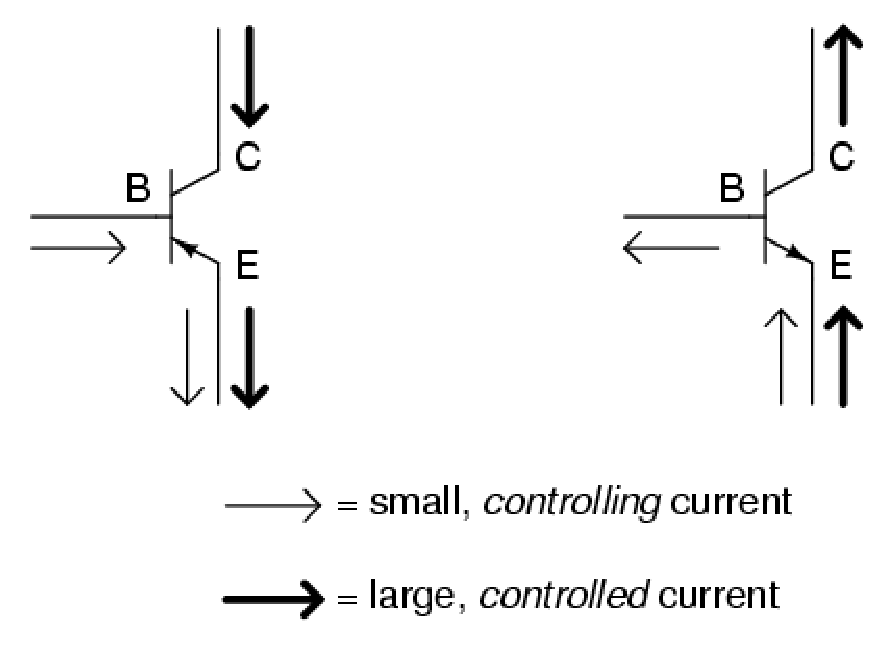
\includegraphics[scale=0.7]{../../epsimages/tranistorcurrents.eps}
\caption{An overview of bipolar transistors as current amplifiers. (Left) An NPN transistor. (Right) A PNP transistor.}
\label{fig:transcur}
\end{center}
\end{figure}

\begin{IFact}{The transistor is considered by many to be one of the greatest discoveries or inventions in modern history, ranking with banking and the printing press. Key to the importance of the transistor in modern society is its ability to be produced in huge numbers using simple techniques, resulting in vanishingly small prices. Computer ``chips'' consist of millions of transistors and sell for Rands, with per-transistor costs in the thousandths-of-cents. The low cost has meant that the transistor has become an almost universal tool for non-mechanical tasks. Whereas a common device, say a refrigerator, would have used a mechanical device for control, today it is often less expensive to simply use a few million transistors and the appropriate computer program to carry out the same task through "brute force". Today transistors have replaced almost all electromechanical devices, most simple feedback systems, and appear in huge numbers in everything from computers to cars.}\end{IFact} 

\begin{IFact}{The transistor was invented at Bell Laboratories in December 1947 (first demonstrated on December 23) by John Bardeen, Walter Houser Brattain, and William Bradford Shockley, who were awarded the Nobel Prize in physics in 1956.}\end{IFact}

\subsubsection{The Field Effect Transistor (FET)}

To control a bipolar transistor, you control the {\bf current} flowing into or out of its base.  The other type of transistor is the field effect transistor (FET).  FETs work using control {\bf voltages} instead.  Accordingly they can be controlled with much smaller currents and are much more economic to use.  

\begin{IFact}{No-one would build a computer with billions of bipolar transistors --- the current in each transistor's base might be small, but when you add up all of the base currents in the millions of transistors, the computer as a whole would be consuming a great deal of electricity and making a great deal of heat.  Not only is this wasteful, it would prevent manufacturers making a computer of convenient size.  If the transistors were too close together, they would overheat.}\end{IFact}

\begin{figure}[htbp]
\begin{center} \begin{tabular}{cc}
\begin{pspicture}(0,1)(7,3.3)
\psframe(2,2)(5,3)
\uput[r](1.9,2.5){N}
\uput[r](4.4,2.5){N}
\psframe(2.5,2)(4.5,2.5)
\uput[r](3.3,2.3){P}
\uput[r](2.8,2.8){Channel}
\psline(0,2.5)(2,2.5)
\uput[r](0.0,2.7){Source}
\psline(5,2.5)(7,2.5)
\uput[r](6,2.7){Drain}
\psline(3.5,2)(3.5,1.2)(5.5,1.2)
\uput[r](5.2,1.4){Gate}
\end{pspicture} &
\begin{pspicture}(0,0.8)(5,4)
\pscircle(2,2){0.8}
\psline(0.5,1.5)(1.8,1.5)(1.8,2.5)
\psline(1.8,2.3)(2.2,2.3)(2.2,3.5)
\psline(1.8,1.7)(2.2,1.7)(2.2,0.9)
\uput[r](0.2,1.7){Gate}
\uput[r](2.1,1){Source}
\uput[r](2.1,3.6){Drain}
\end{pspicture} \\
\end{tabular}
\caption{A field effect transistor (FET).  The diagram on the left shows the semiconductor structure.  The diagram on the right shows its circuit symbol.}
\label{fig:fet}
\end{center}
\end{figure}

The three terminals of the FET are called the \textit{source} (S), \textit{drain} (D) and \textit{gate} (G), as shown in Figure~\ref{fig:fet}.  When the gate is not connected, a current of electrons can flow from source (S) to drain (D) easily along the channel.  The source is, accordingly, the negative terminal of the transistor.  The drain, where the electrons come out, is the positive terminal of the transistor.  A few electrons will flow from the n-type channel into the p-type semiconductor of the gate when the device is manufactured.  However, as these electrons are not removed (the gate is not connected), a depletion band is set up which prevents further flow into the gate.

In operation, the gate is connected to negative voltages relative to the source.  This makes the p-n junction between gate and channel reverse-biased.  Accordingly no current flows from the source into the gate.  When the voltage of the gate is lowered (made more negative), the depletion band becomes wider.  This enlarged depletion band takes up some of the space of the channel.  So the lower the voltage of the gate (the more negative it is relative to the source), the larger the depletion band.  The larger the depletion band, the narrower the channel.  The narrower the channel, the harder it is for electrons to flow from source to drain.

The voltage of the gate is not the only factor affecting the current of electrons between the source and the drain.  If the external circuit has a low resistance, electrons are able to leave the drain easily.  If the external circuit has a high resistance, electrons leave the drain slowly.  This creates a kind of `traffic jam' which slows the passage of further electrons.  In this way, the voltage of the drain regulates itself, and is more or less independent of the current demanded from the drain.

Once these two factors have been taken into account, it is fair to say that the positive output voltage (the voltage of the drain relative to the source) is proportional to the negative input voltage (the voltage of the gate relative to the source).

For this reason, the field effect transistor is known as a voltage amplifier.  This contrasts with the bipolar transistor which is a current amplifier.

\Exercise{Field Effect Transistors}{
\begin{enumerate}
\item What are the two types of bipolar transistor?  How does their construction differ?
\item What are the three connections to a bipolar transistor called?
\item Why are very few electrons able to flow from emitter to collector in an NPN transistor if the base is not connected?
\item Why do you think a bipolar transistor would not work if the base layer were too thick?
\item ``The bipolar transistor is a current amplifier.''  What does this statement mean?
\item Describe the structure of a FET.
\item Define what is meant by the source, drain and gate.  During normal operation, what will the voltages of drain and gate be with respect to the source?
\item Describe how a depletion layer forms when the gate voltage is made more negative. What controls the width of the depletion layer?
\item ``The field effect transistor is a voltage amplifier.'' What does this statement mean?
\item The amplifier in a cheap radio will probably contain bipolar transistors.  A computer contains many field effect transistors.  Bipolar transistors are more rugged and less sensitive to interference than field effect transistors, which makes them more suitable for a simple radio.  Why are FETs preferred for the computer?
\end{enumerate}}

\subsection{The Operational Amplifier}
%\begin{syllabus}
%\item The learner must be able to Explain that for mathematical operations such as multiplication and addition, a special amplifier is required.  Such a device is an operational amplifier or op-amp.
%\item Use the 741 op-amp as an example and explain that it has two input terminals called the inverting and non-inverting inputs.
%\item  Explain the need for a trimming potentiometer when using an op-amp.
%\end{syllabus}

The operational amplifier is a special kind of voltage amplifier which is made from a handful of bipolar or field effect transistors.  Operational amplifiers are usually called {\bf op-amps} for short.  They are used extensively in all kinds of audio equipment (amplifiers, mixers and so on) and in instrumentation.  They also have many other uses in other circuits - for example comparing voltages from sensors.

Operational amplifiers are supplied on Integrated Circuits (I.C.s).  The most famous operational amplifier I.C. is numbered 741 and contains a single operational amplifier on an integrated circuit (`chip') with eight terminals.  Other varieties can be bought, and you can get a single integrated circuit with two or four `741'-type operational amplifiers on it.

The symbol for an op-amp is shown in Figure~\ref{fig:opamp}. The operational amplifier has two input terminals and one output terminal.  The voltage of the output terminal is proportional to the difference in voltage between the two input terminals.  The output terminal is on the right (at the sharp point of the triangle).  The two input terminals are drawn on the left.  
One input terminal (labelled with a $+$ on diagrams) is called the {\bf non-inverting input}.  The other input terminal (labelled $-$) is called the {\bf inverting input}.  The labels $+$ and $-$ have nothing to do with the way in which the operational amplifier is connected to the power supply.  Operational amplifiers must be connected to the power supply, but this is taken for granted when circuit diagrams are drawn, and these connections are not shown on circuit diagrams.  Usually, when drawing electronic circuits, `0V' is taken to mean the negative terminal of the power supply.  This is not the case with op-amps.  For an op-amp, `0V' refers to the voltage midway between the $+$ and $-$ of the supply.

\begin{figure}[H]
\begin{center}
\begin{pspicture}(0,-0.6)(5,3.6)
%\psgrid[gridcolor=gray]
\pnode(0,0){A}
\pnode(0,3){B}
\pnode(5,1.5){C}
\OA(B)(A)(C)
\uput[dr](0,0){non-inverting input terminal}
\uput[ur](0,3){inverting input terminal}
\uput[r](5,1.5){output terminal}
\end{pspicture}
\caption{Circuit symbol for an operational amplifier.  The amplifier must also be connectd to the $+$ and $-$ terminals of the power supply.  These connections are taken for granted and not shown.}
\label{fig:opamp}
\end{center}
\end{figure}

The output voltage of the amplifier $V_{out}$ is given by the formula
\equ{V_{out} = A \left( V_{+} - V_{-} \right)}
where $A$ is a constant called the {\bf open loop gain}, and $V_{+}$ and $V_{-}$ are the voltages of the two input terminals.  That said, the output voltage can not be less than the voltage of the negative terminal of the battery supplying it or higher than the positive terminal of the battery supplying it.  You will notice that $V_{out}$ is positive if $V_{+} > V_{-}$ and negative if $V_{+} < V_{-}$.  This is why the $-$ input is called the inverting input: raising its voltage causes the output voltage to {\it drop}.

The input resistance of an operational amplifier is very high.  This means that very little current flows into the input terminals during operation.

If all of the transistors in the operational amplifier were identical then the output voltage would be zero if the two inputs were at equal voltages.  In practice this is not quite the case, and for sensitive work a {\bf trimming potentiometer} is connected.  This is adjusted until the op-amp is zeroed correctly.  

Simple operational amplifiers require the trimming potentiometer to be built into the circuit containing them, and an example is shown in Figure~\ref{fig:invertamplifier}.  Other operational amplifier designs incorporate separate terminals for the trimming potentiometer.  These special terminals are labelled {\bf offset} on the manufacturer's diagram.  The exact method of connecting the potentiometer to the offset terminals can depend on the design of the operational amplifier, and you need to refer to the manufacturer's data sheet for details of which potentiometer to use and how to connect it.

For most commercially produced operational amplifiers (known as op-amps for short), the open loop gain $A$ is very large and does not stay constant.  Values of 100 000 are typical.  Usually a designer would want an amplifier with a stable gain of smaller value, and builds the operational amplifier into a circuit like the one in Figure~\ref{fig:invertamplifier}.


\begin{figure}[H]
\begin{center}
\begin{pspicture}(1,1)(10,7)
\psline(4,4)(4,6)(5.5,5)(4,4)
\uput[r](3.9,4.5){$+$}
\uput[r](3.9,5.5){$-$}
\psframe(2.5,5.3)(3.5,5.7)
\uput[r](2.6,5.9){$R_{1}$}
\psframe(4.2,6.5)(5.2,6.9)
\uput[r](4.3,7.1){$R_{2}$}
\psline(1.5,5.5)(2.5,5.5)
\uput[r](1.3,5.7){Input}
\psline(3.5,5.5)(4,5.5)
\psline(5.5,5)(7.5,5)
\uput[r](6.5,5.2){Output}
\psline(3.7,5.5)(3.7,6.7)(4.2,6.7)
\psline(5.2,6.7)(5.7,6.7)(5.7,5)

\psframe(2.8,1.5)(3.2,2.5)
\uput[r](2.1,2.0){$R_{3}$}
\psline{<-}(3.2,2)(3.7,2)
\psline(3.7,2)(3.7,4.5)(4,4.5)

\psline(1,2.2)(2,2.2)
\uput[r](1,2.4){$+$}
\psline(1.3,2)(1.7,2)
\psline(1.5,2.2)(1.5,3)(3,3)(3,2.5)
\psline(1.5,2)(1.5,1)(3,1)(3,1.5)
\end{pspicture}
\caption{An inverting amplifier built using an operational amplifier.  The connections from battery to operational amplifier are not shown.  The output voltage $V_{out} = - R_{2} V_{in} / R_{1}$, as explained in the text.  The potentiometer $R_{3}$ is a trimming potentiometer.  To set it, the input is connected to zero volts.  The trimming potentiometer is then adjusted until $V_{out} = 0$.  In all operational amplifier circuits, zero volts is midway between the $+$ and $-$ of the supply.}
\label{fig:invertamplifier}
\end{center}
\end{figure}



\Extension{Calculating the gain of the amplifier in Figure~\ref{fig:invertamplifier}.}{
\begin{enumerate}
\item The input resistance of the operational amplifier is very high.  This means that very little current flows into the inverting input of the op-amp.  Accordingly, the current through resistor $R_{1}$ must be almost the same as the current through resistor $R_{2}$.  This means that the ratio of the voltage across $R_{1}$ to the voltage across $R_{2}$ is the same as the ratio of the two resistances.
\item The open loop gain $A$ of the op-amp is very high.  Assuming that the output voltage is less than a few volts, this means that the two input terminals must be at very similar voltages.  We shall assume that they are at the same voltage.  
\item We want the output voltage to be zero if the input voltage is zero.  Assuming that the transistors within the op-amp are very similar, the output voltage will only be zero for zero input voltage if $V_{+}$ is very close to zero.  We shall assume that $V_{+}=0$ when the trimming potentiometer is correctly adjusted.
\item It follows from the last two statements that $V_{-} \approx 0$, and we shall assume that it is zero.
\item With these assumptions, the voltage across $R_{2}$ is the same as $V_{out}$, and the voltage across $R_{1}$ is the same as $V_{in}$.  Since both resistors carry the same current (as noted in point 1), we may say that the magnitude of $V_{out} / V_{in} = R_{2} / R_{1}$.  However, if $V_{in}$ is negative, then $V_{out}$ will be positive.  Therefore it is customary to write the gain of this circuit as $V_{out} / V_{in} = - R_{2} / R_{1}$.
\end{enumerate}}




\Exercise{Operational Amplifiers}{
\begin{enumerate}
\item What are operational amplifiers used for?
\item Draw a simple diagram of an operational amplifier and label its terminals.
\item  Why is a trimming potentiometer needed when using an op-amp?
\end{enumerate}}

\section{The Principles of Digital Electronics}
%\begin{syllabus}
%\item The learner must be able to Describe digital electronics as all-pervasive in modern technology: it is the ability to encode information with digital symbols that has made information processing the most important of modern technologies.
%\item The learner must be able to State that in digital electronics, two symbols are used: 1, which means "high" and 0, which means "low" (binary system).
%\item The learner must be able to Describe a logic gate as a device made with groups of transistors on a single chip called an integrated circuit (IC).
%\item The learner must be able to Recall the five main types of logic gates: i.e. NOT;  AND;  OR;  NAND;  NOR. Illustrate the correct symbol for each logic gate.
%\item The learner must be able to Compile the relevant truth table for each of the five logic gates.
%\item The learner must be able to Perform simple problem-solving exercises with two gates joined together to find the equivalent gate using truth tables.
%\item The learner must be able to Describe and explain how to use transistors to make a circuit that can count in the binary system.
%\end{syllabus}

The circuits and components we have discussed are very useful.  You can build a radio or television with them.  You can make a telephone.  Even if that was all there was to electronics, it would still be very useful.  However, the great breakthrough in the last fifty years or so has been in {\bf digital} electronics.  This is the subject which gave us the computer.  The computer has revolutionized the way business, engineering and science are done.  Small computers programmed to do a specific job (called microprocessors) are now used in almost every electronic machine from cars to washing machines.  Computers have also changed the way we communicate.  We used to have telegraph or telephone wires passing up and down a country --- each one carrying one telephone call or signal.  We now have optic fibres each capable of carrying tens of thousands of telephone calls using {\bf digital} signals.


So, what is a digital signal?  Look at Figure~\ref{fig:digitalanalogue}.  A normal signal, called an {\bf analogue} signal, carries a smooth wave.  At any time, the voltage of the signal could take any value.  It could be 2,00 V or 3,53 V or anything else.  A digital signal can only take certain voltages.  The simplest case is shown in the figure --- the voltage takes one of two values.  It is either {\bf high}, or it is {\bf low}.  It never has any other value.

These two special voltages are given symbols.  The low voltage level is written 0, while the high voltage level is written as 1.  When you send a digital signal, you set the voltage you want (0 or 1), then keep this fixed for a fixed amount of time (for example 0.01 $\mu$s), then you send the next 0 or 1.  The digital signal in Figure~\ref{fig:digitalanalogue} could be written 01100101.


\begin{figure}[H]
\begin{center}
\begin{pspicture}(0,-1)(12,6)
\psline[arrows=->](0,0)(5,0)
\uput[r](4,-0.2){time}
\psline[arrows=->](0,0)(0,4)
\uput[r](2,4.3){Analogue}

\pscurve(0,0)(1,3)(1.5,2)(2,2.5)(3,1.1)(3.5,0.3)(4,1.3)(4.5,2.4)(5,1.5)

\psline[arrows=->](7,0)(12,0)
\uput[r](11,-0.2){time}
\psline[arrows=->](7,0)(7,4)
\uput[r](9,4.3){Digital}

\uput[r](7.0,2){0}
\psline(7.5,0)(7.5,4)
\uput[r](7.5,2){1}
\uput[r](8.0,2){1}
\psline(7.5,4)(8.5,4)
\psline(8.5,0)(8.5,4)
\uput[r](8.5,2){0}
\uput[r](9.0,2){0}
\psline(9.5,0)(9.5,4)
\psline(9.5,4)(10.0,4)
\uput[r](9.5,2){1}
\psline(10.0,4)(10,0)
\uput[r](10.0,2){0}
\psline(10.5,0)(10.5,4)
\psline(10.5,4)(11,4)
\uput[r](10.5,2){1}
\end{pspicture}
\caption{The difference between normal (analogue) signals and digital signals. }
\label{fig:digitalanalogue}
\end{center}
\end{figure}

Why are digital signals so good?
\begin{enumerate}
\item Using a computer, any information can be turned into a pattern of 0s and 1s.  Pictures, recorded music, text and motion pictures can all be turned into a string of 0s and 1s and transmitted or stored in the same way.  The computer receiving the signal at the other end converts it back again.  A Compact Disc (CD) for example, can store music or text or pictures, and all can be read using a computer.
\item The 0 and the 1 look very different.  You can immediately tell if a 0 or a 1 is being sent.  Even if there is interference, you can still tell whether the sender sent a 0 or a 1.  This means that fewer mistakes are made when reading a digital signal.  This is why the best music recording technologies, and the most modern cameras, for example, all use digital technology.
\item Using the 0s and 1s you can count, and do all kinds of mathematics.  This will be explained in more detail in the next section.
\end{enumerate}

The simplest digital circuits are called {\bf logic gates}.  Each logic gate makes a decision based on the information it receives.  Different logic gates are set up to make the decisions in different ways.  Each logic gate will be made of many microscopic transistors connected together within a thin wafer of silicon.  This tiny circuit is called an Integrated Circuit or I.C. - all the parts are in one place (integrated) on the silicon wafer.  

\subsection{Logic Gates}
There are five main types of logic gate: NOT, AND, OR, NAND and NOR. Each one makes its decision in a different way.


\subsubsection{The NOT Gate}
{\bf Problem:} You want an automatic circuit in your office to turn on the heating in the winter.  You already have a digital electronic temperature sensor.  When the temperature is high, it sends out a 1.  When the office is cold, it sends out a 0.  If this signal were sent straight to the heater, the heater would turn on (1) when it was already hot, and would stay off when it was cold.  This is wrong!  To make the heater work, we need a circuit which will change a 0 (from the sensor) into a 1 (to send to the heater).  This will make the heater come on when it is cold. You also want it to change a 1 (from the sensor) into a 0 (to send to the heater).  This will turn the heater off when the room is hot.  This circuit is called an {\bf inverter} or {\bf NOT gate}.  It changes 0 into 1 (1 is NOT 0).  It changes 1 into 0 (0 is NOT 1).  It changes a signal into what it is NOT.

The symbol for the NOT gate is:

\begin{center}
\begin{pspicture}(0,0)(2.2,1.7)
\psline(0.5,0)(0.5,1)(1.5,0.5)(0.5,0)
\pscircle(1.6,0.5){0.1}
\psline(0,0.5)(0.5,0.5)
\psline(1.7,0.5)(2.5,0.5)
\end{pspicture}
\end{center}

The action of the NOT gate can be written in a table called a {\bf truth table}.  The left column shows the possible inputs on different rows.  The right column shows what the output (decision) of the circuit will be for that input.  The truth table for the NOT gate is shown below.

\begin{center}
\begin{tabular}{|c|c|}\hline
\textbf{Input} & \textbf{Output}\\\hline\hline
0&1\\\hline
1&0\\\hline
\end{tabular}
\end{center}

When you read the truth table, the top row says, ``If the input is 0, the output will be 1.''  For our heater, this means, ``If the room is cold, the heater will turn on.''  The bottom row says, ``If the input is 1, the output will be 0.''  For our heater, this means, ``If the room is hot, the heater will switch off.''

\subsubsection{The AND Gate}
{\bf Problem:} An airliner has two toilets.  Passengers get annoyed if they get up from their seat only to find that both toilets are being used and they have to go back to their seat and wait.  You want to fit an automatic circuit to light up a display if both toilets are in use.  Then passengers know that if the light is off, there will be a free toilet for them to use.  There is a sensor in each toilet.  It gives out a 0 of the toilet is free, and a 1 if it is in use.  You want to send a 1 to the display unit if {\bf both} sensors are sending 1s.  To do this, you use an AND gate.

The symbol for the AND gate is:

\begin{figure}[htbp]
\begin{center}
\begin{pspicture}(1.5,0)(4.5,2)
\psline(2.7,1.8)(2,1.8)(2,0.2)(2.7,0.2)
\psarc(2.7,1){0.8}{-90}{90}
\psline(1.5,0.5)(2,0.5)
\psline(1.5,1.5)(2,1.5)
\psline(3.5,1)(4.2,1)
\end{pspicture}
\caption{Symbol for the AND logic gate.}
\end{center}
\end{figure}

The truth table for the AND gate is shown below.  An AND gate has two inputs (the NOT gate only had one).  This means we need four rows in the truth table, one for each possible set of inputs.  The first row, for example, tells us what the AND gate will do if both inputs are 0.  In our airliner, this means that both toilets are free.  The right column has a 0 showing that the output will be 0, so the display will not light up.  The second row has inputs of 0 and 1 (the first toilet is free, the other is in use).  Again the output is 0.  The third row tells us what will happen if the inputs are 1 and 0 (the first toilet is in use, and the second is free).  Finally, the last line tells us what will happen if both inputs are 1 (the first toilet is in use and the second toilet is in use).  It is only in this case that the output is 1 and the display lights up.

\begin{center}
\begin{tabular}{|c|c|c|}\hline
\multicolumn{2}{|c|}{\textbf{Inputs}} & \textbf{Output}\\\hline
A&B& \\\hline\hline
0&0&0\\\hline
0&1&0\\\hline
1&0&0\\\hline
1&1&1\\\hline
\end{tabular}
\end{center}

This device is called an AND gate, because the output is only 1 if one input AND the other input are both 1.

\Extension{Using 0 and 1 to mean True and False}{When we use logic gates we use the low voltage state 0 to represent `false'.  The high voltage state 1 represents `true'.  This is why the word AND is so appropriate.  A AND B is true (1) if, and only if, A is true (1) AND B is true (1).}

\Extension{AND and multiplication}{Sometimes, the AND operation is written as multiplication.  A AND B is written AB.  If either A or B are 0, then AB will also be 0.  For AB to be 1, we need A and B to both be 1.  Multiplication of the numbers 0 and 1 does exactly the same job as an AND gate.}

\subsubsection{The NAND Gate}
{\bf Problem:} You build the circuit for the airliner toilets using an AND gate.  Your customer is pleased, but she says that it would be better if the display lit up when there {\bf was} a free toilet.  In other words, the display should light up unless both toilets are in use.  To do this we want a circuit which does the opposite of an AND gate.  We want a circuit which would give the output 0 where an AND gate would give 1.  We want a circuit which would give the output 1 where an AND gate would give 0.  This circuit is called a NAND gate.

The symbol for the NAND gate is:

\begin{figure}[H]
\begin{center}
\begin{pspicture}(1.5,0)(4.5,2)
\psline(2.7,1.8)(2,1.8)(2,0.2)(2.7,0.2)
\psarc(2.7,1){0.8}{-90}{90}
\pscircle(3.6,1){0.1}
\psline(1.5,0.5)(2,0.5)
\psline(1.5,1.5)(2,1.5)
\psline(3.7,1)(4.2,1)
\end{pspicture}
%\caption{Symbol for the NAND logic gate.}
\end{center}
\end{figure}

The truth table for the NAND gate is shown below.

\begin{center}
\begin{tabular}{|c|c|c|}\hline
\multicolumn{2}{|c|}{\textbf{Inputs}} & \textbf{Output}\\\hline
A&B& \\\hline\hline
0&0&1\\\hline
0&1&1\\\hline
1&0&1\\\hline
1&1&0\\\hline
\end{tabular}
\end{center}

You may have noticed that we could have done this job on the airliner by using our earlier circuit, with a NOT gate added between the original AND gate and the display.  This is where the word NAND comes from --- it is short for NotAND.

\subsubsection{The OR Gate}
{\bf Problem:} A long, dark corridor has two light switches --- one at each end of the corridor.  The switches each send an output of 0 to the control unit if no-one has pressed the switch.  If someone presses the switch, its output is 1.  The lights in the corridor should come on if either switch is pressed. To do this job, the control unit needs an OR gate. The symbol for the OR gate is:

\begin{figure}[H]
\begin{center}
\begin{pspicture}(1.5,0)(4.5,2)

\pscurve(2,0.2)(2.2,1)(2,1.8)
\pscurve(2,1.8)(3,1.5)(3.5,1)
\pscurve(2,0.2)(3,0.5)(3.5,1)

\psline(1.5,0.5)(2,0.5)
\psline(1.5,1.5)(2,1.5)
\psline(3.5,1)(4.2,1)
\end{pspicture}
\caption{Symbol for the OR logic gate.}
\end{center}
\end{figure}

The truth table for the OR gate is shown.

\begin{center}
\begin{tabular}{|c|c|c|}\hline
\multicolumn{2}{|c|}{\textbf{Inputs}} & \textbf{Output}\\\hline
A&B& \\\hline\hline
0&0&0\\\hline
0&1&1\\\hline
1&0&1\\\hline
1&1&1\\\hline
\end{tabular}
\end{center}

You can see that the output is 1 (and the lights come on in the corridor) if either one switch OR the other is pressed.  Pressing both switches also turns on the lights, as the last row in the table shows.

\Extension{OR and addition}{Sometimes you will see A OR B written mathematically as A+B.  This makes sense, since if A=0 and B=0, then A OR B = A+B = 0.  Similarly, if A=0 and B=1, then A OR B = A+B = 1.  If A=1 and B=0, then A OR B = A+B = 1 once again.  The only case where the OR function differs from normal addition is when A=1 and B=1.  Here A OR B = 1 in logic, but A+B=2 in arithmetic.  However, there is no such thing as `2' in logic, so we define + to mean `OR', and write 1+1=1 with impunity!


If you wish, you can prove that the normal rules of algebra still work using this notation:  A+(B+C) = (A+B)+C, A(BC) = (AB)C, and A(B+C) = AB + AC.  This special kind of algebra where variables can only be 0 (representing false) or 1 (representing true) is called Boolean algebra.}

\subsubsection{The NOR Gate}
The last gate you need to know is the NOR gate.  This is opposite to the OR gate.  The output is 1 if both inputs are 0.  In other words, the output switches on if neither the first NOR the second input is 1.  The symbol for the NOR gate is:

\begin{figure}{H}
\begin{center}
\begin{pspicture}(1.5,0)(4.5,2)

\pscurve(2,0.2)(2.2,1)(2,1.8)
\pscurve(2,1.8)(3,1.5)(3.5,1)
\pscurve(2,0.2)(3,0.5)(3.5,1)
\pscircle(3.6,1){0.1}
\psline(1.5,0.5)(2,0.5)
\psline(1.5,1.5)(2,1.5)
\psline(3.7,1)(4.2,1)
\end{pspicture}
\caption{Symbol for the NOR logic gate.}
\end{center}
\end{figure}

The truth table for the NOR gate is shown below.

\begin{center}
\begin{tabular}{|c|c|c|}\hline
\multicolumn{2}{|c|}{\textbf{Inputs}} & \textbf{Output}\\\hline
A&B& \\\hline\hline
0&0&1\\\hline
0&1&0\\\hline
1&0&0\\\hline
1&1&0\\\hline
\end{tabular}
\end{center}

The examples given were easy.  Each job only needed one logic gate.  However any `decision making' circuit can be built with logic gates, no matter how complicated the decision.  Here is an example.

\begin{wex}{An Economic Heating Control}{A sensor in a building detects whether a room is being used. If it is empty, the output is 0, if it is in use, the output is 1.  Another sensor measures the temperature of the room.  If it is cold, the output is 0.  If it is hot, the output is 1.  The heating comes on if it receives a 1.  Design a control circuit so that the heating only comes on if the room is in use and it is cold.}{The first sensor tells us whether the room is occupied.  The second sensor tells us whether the room is hot.  The heating must come on if the room is occupied AND cold.  This means that the heating should come on if the room is occupied AND (NOT hot).  To build the circuit, we first attach a NOT gate to the output of the temperature sensor.  This output of the NOT gate will be 1 only if the room is cold.  We then attach this output to an AND gate, together with the output from the other sensor. The output of the AND gate will only be 1 if the room is occupied AND the output of the NOT gate is also 1.  So the heating will only come on if the room is in use and is cold.  The circuit is shown below.

\begin{center}
\begin{pspicture}(0,0)(5.2,2)
\psline(2.7,1.8)(2,1.8)(2,0.2)(2.7,0.2)
\psarc(2.7,1){0.8}{-90}{90}
\psline(0,0.5)(2,0.5)
\uput[r](0,0.1){Occupied}
\psline(0,1.5)(0.9,1.5)
\uput[r](0,1.7){Hot}
\psline(0.9,1.8)(0.9,1.2)(1.5,1.5)(0.9,1.8)
\pscircle(1.6,1.5){0.1}
\psline(1.7,1.5)(2,1.5)
\psline(3.5,1)(4.2,1)
\uput[r](4.3,1){Output}
\end{pspicture}
\end{center}}
\end{wex}


\begin{wex}{Solving a circuit with two logic gates}{Compile the truth table for the circuit below.

\begin{center}
\begin{pspicture}(1.5,0)(6,2)
\pscurve(2,0.2)(2.2,1)(2,1.8)
\pscurve(2,1.8)(3,1.5)(3.5,1)
\pscurve(2,0.2)(3,0.5)(3.5,1)
\pscircle(3.6,1){0.1}
\psline(1.5,0.5)(2,0.5)
\psline(1.5,1.5)(2,1.5)
\psline(3.7,1)(4.2,1)
\psline(4.2,0.5)(4.2,1.5)(5.2,1)(4.2,0.5)
\pscircle(5.3,1){0.1}
\psline(5.4,1)(5.9,1)
\end{pspicture}
\end{center}
}{Firstly, we label the inputs A and B.  We also label the point where the two gates are connected C.
\begin{center}
\begin{pspicture}(1.2,0)(6.3,2)
\pscurve(2,0.2)(2.2,1)(2,1.8)
\pscurve(2,1.8)(3,1.5)(3.5,1)
\pscurve(2,0.2)(3,0.5)(3.5,1)
\pscircle(3.6,1){0.1}
\uput[r](0.9,0.5){A}
\psline(1.5,0.5)(2,0.5)
\uput[r](0.9,1.5){B}
\psline(1.5,1.5)(2,1.5)
\psline(3.7,1)(4.2,1)
\uput[r](3.6,1.2){C}
\psline(4.2,0.5)(4.2,1.5)(5.2,1)(4.2,0.5)
\pscircle(5.3,1){0.1}
\psline(5.4,1)(5.9,1)
\uput[r](5.5,1.2){Output}
\end{pspicture}
\end{center}
Next we prepare a truth table.  There is a column for each of the inputs, for the intermediate point C and also for the output.  The truth table has four rows, since there are four possible inputs --- 00, 01, 10 and 11.
\begin{center}
\begin{tabular}{|c|c|c|c|}\hline
A&B&C&Output\\\hline\hline
0&0& & \\\hline
0&1& & \\\hline
1&0& & \\\hline
1&1& & \\\hline
\end{tabular}
\end{center}
Next we fill in the C column given that we know what a NOR gate does.
\begin{center}
\begin{tabular}{|c|c|c|c|}\hline
A&B&C&Output\\\hline\hline
0&0&1& \\\hline
0&1&0& \\\hline
1&0&0& \\\hline
1&1&0& \\\hline
\end{tabular}
\end{center}
Next, we can fill in the output, since it will always be the opposite of C (because of the NOT gate).
\begin{center}
\begin{tabular}{|c|c|c|c|}\hline
A&B&C&Output\\\hline\hline
0&0&1&0\\\hline
0&1&0&1\\\hline
1&0&0&1\\\hline
1&1&0&1\\\hline
\end{tabular}
\end{center}
Finally we see that this combination of gates does the same job as an OR gate.
}
\end{wex}

Each logic gate is manufactured from two or more transistors.  Other circuits can be made using logic gates, as we shall see in the next section.  We shall show you how to count and store numbers using logic gates.  This means that if you have enough transistors, and you connect them correctly to make the right logic gates, you can make circuits which count and store numbers.

In practice, the cheapest gate to manufacture is usually the NAND gate. Additionally, Charles Peirce showed that NAND gates alone (as well as NOR gates alone) can be used to reproduce all the other logic gates.

\Exercise{The Principles of Digital Electronics}{
\begin{enumerate}
\item Why is digital electronics important to modern technology and information processing?
\item What two symbols are used in digital electronics, to represent a ``high" and a ``low"? What is this system known as?
\item What is a logic gate?
\item What are the five main types of logic gates? Draw the symbol for each logic gate.
\item Write out the truth tables for each of the five logic gates.
\item Write out the truth table for the following circuit.  Which single gate is this circuit equivalent to?
\begin{center}
\begin{pspicture}(1.5,0)(6.5,2)
\psline(2.7,1.8)(2,1.8)(2,0.2)(2.7,0.2)
\psarc(2.7,1){0.8}{-90}{90}
\pscircle(3.6,1){0.1}
\psline(1.5,0.5)(2,0.5)
\psline(1.5,1.5)(2,1.5)
\psline(3.7,1)(4.2,1)
\psline(4.2,1.5)(4.2,0.5)(5.2,1)(4.2,1.5)
\pscircle(5.3,1){0.1}
\psline(5.4,1)(6.4,1)
\end{pspicture}
\end{center}
\item Write out the truth table for the following circuit.  Which single gate is this circuit equivalent to?
\begin{center}
\begin{pspicture}(0,0)(4.5,2)

\pscurve(2,0.2)(2.2,1)(2,1.8)
\pscurve(2,1.8)(3,1.5)(3.5,1)
\pscurve(2,0.2)(3,0.5)(3.5,1)

\psline(1.5,0.5)(2,0.5)
\psline(1.5,1.5)(2,1.5)
\psline(3.5,1)(4.2,1)

\psline(1.3,0.5)(0.7,0.8)(0.7,0.2)(1.3,0.5)
\pscircle(1.4,0.5){0.1}
\psline(0,0.5)(0.7,0.5)

\psline(1.3,1.5)(0.7,1.8)(0.7,1.2)(1.3,1.5)
\pscircle(1.4,1.5){0.1}
\psline(0,1.5)(0.7,1.5)
\end{pspicture}
\end{center}
\end{enumerate}}

\section{Using and Storing Binary Numbers}

%\begin{syllabus}
%\item The learner must be able to State that the basis of all computer memories is the bistable or flip-flop.
%\item The learner must be able to Demonstrate and explain that two NOR gates in series form a flip-flop and can remember one bit of information;
%\item The learner must be able to State that one bit is short for binary digit.
%\item The learner must be able to Demonstrate that all numbers can represented as binary numbers and be expressed in terms of 0s and 1s.
%\item The learner must be able to Show that counting circuits use flip-flops to "divide by two".
%\item The learner must be able to Describe that the modulo of a counter is the number of pulses needed to reset its output states to 0.  For example, a modulo counter counts up to seven then resets itself to zero.
%\item The learner must be able to Describe and explain a modulo 8 counter to allow counting from 0 (=000) to 7 (=111) using three flip-flops.
%\item The learner must be able to Explain that computers use millions of NOR gates to count.
%\item The learner must be able to Describe how to use NOR gates to make a circuit that can count
%\end{syllabus}

In the previous section, we saw how the numbers 0 and 1 could represent `false' and `true' and could be used in decision making.  Often we want to program a computer to count with numbers.  To do this we need a way of writing any number using nothing other than 0 and 1.  When written in this way, numbers are called {\bf binary numbers}.

\Definition{Binary Number System}{A way of writing any number using only the digits 0 and 1.}

\subsection{Binary numbers}

In normal (denary) numbers, we write 9+1 as 10.  The fact that the `1' in 10 is the second digit from the right tells us that it actually means 10 and not 1.  Similarly, the `3' in 365 represents 300 because it is the third digit from the right.  You could write 365 as $3 \times 100 + 6 \times 10 + 5$.  You will notice the pattern that the $n$th digit from the right represents $10^{n-1}$.  In binary, we use the $n$th digit from the right to represent $2^{n-1}$.  Thus 2 is written as 10 in binary.  Similarly $2^{2} = 4$ is written as 100 in binary, and $2^{3} = 8$ is written as 1000 in binary.

\begin{wex}{Conversion of Binary Numbers to Denary Numbers}{Convert the binary number 10101 to its denary equivalent.}{We start on the right.  The `1' on the right does indeed represent one.  The next `1' is in the third place from the right, and represents $2^2 = 4$.  The next `1' is in the fifth place from the right and represents $2^4 = 16$.  Accordingly, the binary number 10101 represents 16+4+1 = 21 in denary notation.}
\end{wex}


\begin{wex}{Conversion of Denary Numbers to Binary Numbers}{Convert the decimal number 12 to its binary equivalent.}{Firstly we write 12 as a sum of powers of 2, so 12 = 8+4.  In binary, eight is 1000, and four is 100.  This means that twelve = eight + four must be 1000+100 = 1100 in binary.  You could also write 12 as $1 \times 8 + 1 \times 4 + 0 \times 2 + 0 \times 1 = 1100$ in binary.}
\end{wex}

\begin{IFact}{How do you write numbers as a sum of powers of two?  The first power of two (the largest) is the largest power of two which is not larger than the number you are working with.  In our last example, where we wanted to know what twelve was in binary, the largest power of two which is not larger than 12 is 8.  Thus 12 = 8 + something.  By arithmetic, the `something' must be 4, and the largest power of two not larger than this is 4 exactly.  Thus 12 = 8 + 4, and we have finished.

A more complicated example would be to write one hundred in binary.  The largest power of two not larger than 100 is 64 (1000000 in binary).  Subtracting 64 from 100 leaves 36.  The largest power of two not larger than 36 is 32 (100000 in binary).  Removing this leaves a remainder of 4, which is a power of two itself (100 in binary).  Thus one hundred is 64 + 32 + 4, or in binary  1000000 + 100000 + 100 = 1100100.} \end{IFact}

Once a number is written in binary, it can be represented using the low and high voltage levels of digital electronics.  We demonstrate how this is done by showing you how an electronic counter works.

\subsection{Counting circuits}

To make a counter you need several `T flip flops', sometimes called `divide by two' circuits.  A T flip flop is a digital circuit which swaps its output (from 0 to 1 or from 1 to 0) whenever the input changes from 1 to 0.  When the input changes from 0 to 1 it doesn't change its output.  It is called a {\bf flip flop} because it changes (flips or flops) each time it receives a pulse.

If you put a series of pulses 10101010 into a T flip flop, the result is 01100110.  Figure~\ref{fig:Tinout} makes this clearer.

\begin{figure}[!h]
\begin{center}
\begin{pspicture}(-0.5,-1)(7,6)
\psline[arrows=->](0,0)(6,0)
\uput[r](6,0){time}
\uput[r](1,2.5){Output}

\psline(0.5,0)(0.5,2)
\psline(0.5,2)(1.5,2)
\psline(1.5,2)(1.5,0)
\psline(2.5,0)(2.5,2)
\psline(2.5,2)(3.5,2)
\psline(3.5,2)(3.5,0)

\psline[arrows=->](0,3)(6,3)
\uput[r](6,3){time}
\uput[r](1,5.5){Input}

\psline(0,3)(0,5)
\psline(0,5)(0.5,5)
\psline(0.5,5)(0.5,3)

\psline(1,3)(1,5)
\psline(1,5)(1.5,5)
\psline(1.5,5)(1.5,3)

\psline(2,3)(2,5)
\psline(2,5)(2.5,5)
\psline(2.5,5)(2.5,3)

\psline(3,3)(3,5)
\psline(3,5)(3.5,5)
\psline(3.5,5)(3.5,3)

\end{pspicture}
\caption{The output of a T flip flop, or `divide by two' circuit when a square wave is connected to the input.  The output changes state when the input goes from 1 to 0.}
\label{fig:Tinout}
\end{center}
\end{figure}

As you can see from Figure~\ref{fig:Tinout}, there are half as many pulses in the output.  This is why it is called a `divide by two' circuit.

If we connect T flip flops in a chain, then we make a counter which can count pulses.  As an example, we connect three T flip flops in a chain.  This is shown in Figure~\ref{fig:Tchain}.

\begin{figure}[!h]
\begin{center}
\begin{pspicture}(0,-1)(12,3.2)
\psframe(2,1)(4,3)
\uput[r](1.9,2){T}
\uput[r](3.4,2){Q}
\psline(0,2)(2,2)
\uput[r](0,2.4){Input}

\psframe(5,1)(7,3)
\uput[r](4.9,2){T}
\uput[r](6.4,2){Q}
\psline(4,2)(5,2)
\psline(4.5,2)(4.5,0)
\uput[r](4.2,-0.4){$Q_{0}$}

\psframe(8,1)(10,3)
\uput[r](7.9,2){T}
\uput[r](9.4,2){Q}
\psline(7,2)(8,2)
\psline(7.5,2)(7.5,0)
\uput[r](7.2,-0.4){$Q_{1}$}
\psline(10,2)(10.5,2)(10.5,0)
\uput[r](10.2,-0.4){$Q_{2}$}

\end{pspicture}
\caption{Three T flip flops connected together in a chain to make a counter.  The input of each flip flop is labelled T, while each output is labelled Q.  The pulses are connected to the input on the left.  The outputs $Q_{0}$, $Q_{1}$ and $Q_{2}$ give the three digits of the binary number as the pulses are counted.  This is explained in the text and in the next table.}
\label{fig:Tchain}
\end{center}
\end{figure}

When this circuit is fed with a stream of pulses, the outputs of the different stages change.  The table below shows how this happens.  Each row shows a different stage, with the first stage at the top.  We assume that all of the flip flops have 0 as their output to start with.

\begin{center} \begin{tabular}{|c|c|c|c|r|r|} \hline
Input & Output 1 & Output 2 & Output 3 & Number of pulse & Number in binary \\ \hline
1 & 0 & 0 & 0 & 0 & 000 \\ \hline
0 & 1 & 0 & 0 & 1 & 001 \\ \hline
1 & 1 & 0 & 0 & 1 & 001 \\ \hline
0 & 0 & 1 & 0 & 2 & 010 \\ \hline
1 & 0 & 1 & 0 & 2 & 010 \\ \hline
0 & 1 & 1 & 0 & 3 & 011 \\ \hline
1 & 1 & 1 & 0 & 3 & 011 \\ \hline
0 & 0 & 0 & 1 & 4 & 100 \\ \hline
1 & 0 & 0 & 1 & 4 & 100 \\ \hline
0 & 1 & 0 & 1 & 5 & 101 \\ \hline
1 & 1 & 0 & 1 & 5 & 101 \\ \hline
0 & 0 & 1 & 1 & 6 & 110 \\ \hline
1 & 0 & 1 & 1 & 6 & 110 \\ \hline
0 & 1 & 1 & 1 & 7 & 111 \\ \hline
1 & 1 & 1 & 1 & 7 & 111 \\ \hline
0 & 0 & 0 & 0 & 8 & 1000 \\ \hline
1 & 0 & 0 & 0 & 8 & 1000 \\ \hline
0 & 1 & 0 & 0 & 9 & 1101 \\ \hline
1 & 1 & 0 & 0 & 9 & 1101 \\ \hline \end{tabular} \end{center}
               
The binary numbers in the right hand column count the pulses arriving at the input.  You will notice that the output of the first flip flop gives the right most digit of the pulse count (in binary).  The output of the second flip flop gives the second digit from the right (the `twos' digit) of the pulse count.  The output of the third flip flop gives the third digit from the right (the `fours' digit) of the pulse count.  As there are only three flip flops, there is nothing to provide the next digit (the `eights' digit), and so the eighth pulse is recorded as 000, not 1000.

This device is called a {\bf modulo 8} counter because it can count in eight stages from 000 to 111 before it goes back to 000.  If you put four flip flops in the counter, it will count in sixteen stages from 0000 to 1111, and it is called a modulo 16 counter because it counts in sixteen stages before going back to 0000.

\Definition{Modulo}{The modulo of a counter tells you how many stages (or pulses) it receives before going back to 0 as its output.  Thus a modulo 8 counter counts in eight stages 000, 001, 010, 011, 100, 101, 110, 111, then returns to 000 again.}

\begin{IFact}{If a counter contains $n$ flip flops, it will be a modulo $2^{n}$ counter.  It will count from 0 to $2^{n} - 1$.}\end{IFact}

\subsection{Storing binary numbers}

Counting is important.  However, it is equally important to be able to remember the numbers.  Computers can convert almost anything to a string of 0s and 1s, and therefore to a binary number.  Unless this number can be stored in the computer's memory, the computer would be useless.

The memory in the computer contains many parts.  Each part is able to store a single 0 or 1.  Since 0 and 1 are the two binary digits, we say that each part of the memory stores one {\bf bit}.

\Definition{Bit}{One bit is a short way of saying one `binary digit'.  It is a single 0 or 1.}

\begin{IFact}{If you have eight bits, you can store a binary number from 00000000 to 11111111 (0 to 255 in denary).  This gives you enough permutations of 0s and 1s to have one for each letter of the alphabet (in upper and lower case), each digit from 0 to 9, each punctuation mark and each control code used by a computer in storing a document.  When you type text into a word processor, each character is stored as a set of eight bits.  Each set of eight bits is called a {\bf byte}.  Computer memories are graded according to how many bytes they store.  There are 1024 bytes in a kilobyte (kB), $1024 \times 1024$ bytes in a megabyte (MB), and $1024 \times 1024 \times 1024$ bytes in a gigabyte (GB).} \end{IFact}

To store a bit we need a circuit which can `remember' a 0 or a 1.  This is called a {\bf bistable} circuit because it has two stable states.  It can stay indefinitely either as a 0 or a 1.  An example of a bistable circuit is shown in Figure~\ref{fig:bistable}.  It is made from two NOR gates.

\begin{figure}[!h]
\begin{center}
\begin{tabular}{cc}
\begin{pspicture}(0,0)(6,6)

\pscurve(2,3.2)(2.2,4)(2,4.8)
\pscurve(2,4.8)(3,4.5)(3.5,4)
\pscurve(2,3.2)(3,3.5)(3.5,4)
\pscircle(3.6,4){0.1}

\psline(0.5,4.5)(2,4.5)
\uput[r](0,4.5){R}

\psline(3.7,4)(5,4)
\uput[r](5.2,4){Q}

\psline(4,4)(4,3)(1.5,2)(1.5,1.5)(2,1.5)
\psline[linewidth=0.1cm](3.7,1)(4,1)(4,2)(1.5,3)(1.5,3.5)(2,3.5)

\pscurve(2,0.2)(2.2,1)(2,1.8)
\pscurve(2,1.8)(3,1.5)(3.5,1)
\pscurve(2,0.2)(3,0.5)(3.5,1)
\pscircle(3.6,1){0.1}

\psline(0.5,0.5)(2,0.5)
\uput[r](0,0.5){S}
\end{pspicture} &

\begin{pspicture}(0,0)(6,6)

\pscurve(2,3.2)(2.2,4)(2,4.8)
\pscurve(2,4.8)(3,4.5)(3.5,4)
\pscurve(2,3.2)(3,3.5)(3.5,4)
\pscircle(3.6,4){0.1}

\psline(0.5,4.5)(2,4.5)
\uput[r](0,4.5){R}
\psline[linewidth=0.1cm](3.7,4)(5,4)
\uput[r](5.2,4){Q}

\psline[linewidth=0.1cm](4,4)(4,3)(1.5,2)(1.5,1.5)(2,1.5)
\psline(3.7,1)(4,1)(4,2)(1.5,3)(1.5,3.5)(2,3.5)

\pscurve(2,0.2)(2.2,1)(2,1.8)
\pscurve(2,1.8)(3,1.5)(3.5,1)
\pscurve(2,0.2)(3,0.5)(3.5,1)
\pscircle(3.6,1){0.1}

\psline(0.5,0.5)(2,0.5)
\uput[r](0,0.5){S}
\end{pspicture} \\ 
\end{tabular}
\caption{A bistable circuit made from two NOR gates.  This circuit is able to store one bit of digital information.  With the two inputs set to 0, you can see that the output could be (and will remain) either 0 or 1.  The circuit on the left shows an output of 0, the circuit on the right shows an output of 1.  Wires carrying high logic levels (1) are drawn thicker.  The output of the bistable is labelled Q.}
\label{fig:bistable}
\end{center}
\end{figure}

To store the 0 or the 1 in the bistable circuit, you set one of the inputs to 1, then put it back to 0 again.  If the input labelled `S' (set) is raised, the output will immediately become 1.  This is shown in Figure~\ref{fig:biS}.

\begin{figure}
\begin{center}
\begin{pspicture}(0,0)(6,6)
\pscurve(2,3.2)(2.2,4)(2,4.8)

\pscurve(2,4.8)(3,4.5)(3.5,4)
\pscurve(2,3.2)(3,3.5)(3.5,4)
\pscircle(3.6,4){0.1}

\psline(0.5,4.5)(2,4.5)
\uput[r](0,4.5){R}
\psline[linewidth=0.1cm](3.7,4)(5,4)
\uput[r](5.2,4){Q}

\psline[linewidth=0.1cm](4,4)(4,3)(1.5,2)(1.5,1.5)(2,1.5)
\psline(3.7,1)(4,1)(4,2)(1.5,3)(1.5,3.5)(2,3.5)

\pscurve(2,0.2)(2.2,1)(2,1.8)
\pscurve(2,1.8)(3,1.5)(3.5,1)
\pscurve(2,0.2)(3,0.5)(3.5,1)
\pscircle(3.6,1){0.1}

\psline[linewidth=0.1cm](0.5,0.5)(2,0.5)
\uput[r](0,0.5){S}
\end{pspicture}

\caption{The output of a bistable circuit is {\bf set} (made 1) by raising the `S' input to 1.  Wires carrying high logic levels (1) are shown with thicker lines.}
\label{fig:biS}
\end{center}
\end{figure}

To store a 0, you raise the `R' (reset) input to 1.  This is shown in Figure~\ref{fig:biR}.

\begin{figure}
\begin{center}
\begin{pspicture}(0,0)(6,6)

\pscurve(2,3.2)(2.2,4)(2,4.8)
\pscurve(2,4.8)(3,4.5)(3.5,4)
\pscurve(2,3.2)(3,3.5)(3.5,4)
\pscircle(3.6,4){0.1}

\psline[linewidth=0.1cm](0.5,4.5)(2,4.5)
\uput[r](0,4.5){R}

\psline(3.7,4)(5,4)
\uput[r](5.2,4){Q}

\psline(4,4)(4,3)(1.5,2)(1.5,1.5)(2,1.5)
\psline[linewidth=0.1cm](3.7,1)(4,1)(4,2)(1.5,3)(1.5,3.5)(2,3.5)

\pscurve(2,0.2)(2.2,1)(2,1.8)
\pscurve(2,1.8)(3,1.5)(3.5,1)
\pscurve(2,0.2)(3,0.5)(3.5,1)
\pscircle(3.6,1){0.1}

\psline(0.5,0.5)(2,0.5)
\uput[r](0,0.5){S}
\end{pspicture}

\caption{The output of a bistable circuit is {\bf reset} (made 0) by raising the `R' input to 1. Wires carrying high logic levels (1) are shown with thicker lines.}
\label{fig:biR}
\end{center}
\end{figure}

Once you have used the S or R inputs to set or reset the bistable circuit, you then bring both inputs back to 0.  The bistable `remembers' the state.  Because of the ease with which the circuit can be Reset and Set it is also called an {\bf RS flip flop} circuit.

Computer memory can store millions or billions of bits.  If it used our circuit above, it would need millions or billions of NOR gates, each of which is made from several transistors.  Computer memory is made of many millions of transistors.

\begin{IFact}{The bistable circuits drawn here don't remember 0s or 1s forever --- they lose the information if the power is turned off.  The same is true for the RAM (Random Access Memory) used to store working and temporary data in a computer.  Some modern circuits contain special memory which can remember its state even if the power is turned off.  This is used in FLASH drives, commonly found in USB data sticks and on the memory cards used with digital cameras.  These bistable circuits are much more complex.}  \end{IFact}

You can also make T flip flops out of logic gates, however these are more complicated to design.

\Exercise{Counting Circuits}{
\begin{enumerate}
\item What is the term \textit{bit} short for?
\item What is 43 in binary?
\item What is 1100101 in denary?
\item What is the highest number a modulo 64 counter can count to?  How many T flip flops does it contain?
\item What is the difference between an RS flip flop and a T flip flop?
\item Draw a circuit diagram for a bistable circuit (RS flip flop).  Make three extra copies of your diagram.  On the first diagram, colour in the wires which will carry high voltage levels (digital 1) if the R input is low, and the S input is high.  On the second diagram, colour in the wires which carry high voltage levels if the S input of the first circuit is now made low.  On the third diagram, colour in the wires which carry high voltage levels if the R input is now made high.  On the final diagram, colour in the wires carrying high voltage levels if the R input is now made low again.
\item Justify the statement: a modern computer contains millions of transistors.
\end{enumerate}}


\Exercise{End of Chapter Exercises}{
\begin{enumerate}
\item Calculate the reactance of a 3 mH inductor at a frequency of 50 Hz.
\item Calculate the reactance of a 30 $\mu$F capacitor at a frequency of 1 kHz.
\item Calculate the impedance of a series circuit containing a 5 mH inductor, a 400 $\mu$F capacitor and a 2 k$\Omega$ resistor at a frequency of 50 kHz.
\item Calculate the frequency at which the impedance of the circuit in the previous question will be the smallest.
\item Which component can be used to block low frequencies?
\item Draw a circuit diagram with a battery, diode and resistor in series.  Make sure that the diode is forward biased so that a current will flow through it.
\item When building a complex electronic circuit which is going to be powered by a battery, it is always a good idea to put a diode in series with the battery.  Explain how this will protect the circuit if the user puts the battery in the wrong way round.
\item Summarize the differences betwen a bipolar and field effect transistor.
\item What does an operational amplifier (op-amp) do?
\item What is the difference between a digital signal and an analogue signal?
\item What are the advantages of digital signals over analogue signals?
\item Draw the symbols for the five logic gates, and write down their truth tables.
\item Draw a circuit diagram with an AND gate.  Each input should be connected to the output of a separate NOT gate.  By writing truth tables show that this whole circuit behaves as a NOR gate.
\item Convert the denary number 99 into binary.
\item Convert the binary number 11100111 into denary.
\item Explain how three T flip flops can be connected together to make a modulo 8 counter.  What is the highest number it can count up to?
\item Draw the circuit diagram for an RS flip flop (bistable) using two NOR gates.
\item Show how the circuit you have just drawn can have a stable output of 0 or 1 when both inputs are 0.
\item Operational (and other) amplifiers, logic gates, and flip flops all contain transistors, and would not work without them.  Write a short newspaper article for an intelligent reader who knows nothing about electronics. Explain how important transistors are in modern society.
\end{enumerate}}

% CHILD SECTION END 



% CHILD SECTION START 

\chapter[EM Radiation]{Electromagnetic Radiation}
\label{p:em:emr12}

\section{Introduction}
This chapter will focus on the electromagnetic (EM) radiation. Electromagnetic radiation is a self-propagating wave in space with electric and magnetic components. These components oscillate at right angles to each other and to the direction of propagation, and are in phase with each other. Electromagnetic radiation is classified into types according to the frequency of the wave: these types include, in order of increasing frequency, radio waves, microwaves, infrared radiation, visible light, ultraviolet radiation, X-rays and gamma rays.

\section{Particle/wave nature of electromagnetic radiation}
\label{p:em:emr12:d}
%\begin{syllabus}
%\item Explain that some aspects of the behaviour of EM radiation can best be explained using a wave model and some aspects can best be explained using a particle model
%\item Note: Link to Grade 12 Matter and Materials, photoelectric effect
%\end{syllabus}

If you watch a colony of ants walking up the wall, they look like a thin continuous black line.  But as you look closer, you see that the line is made up of thousands of separated black ants.

Light and all other types of electromagnetic radiation seems like a continuous wave at first, but when one performs experiments with light, one can notice that light can have both wave and particle like properties.  Just like the individual ants, the light can also be made up of individual bundles of energy, or quanta of light.

Light has both wave-like and particle-like properties (wave--particle duality), but only shows one or the other, depending on the kind of experiment we perform. A wave-type experiment shows the wave nature, and a particle-type experiment shows particle nature.  One cannot test the wave and the particle nature at the same time. A particle of light is called a photon.

\Definition{Photon}{A photon is a quantum (energy packet) of light.}

The particle nature of light can be demonstrated by the interaction of photons with matter.  One way in which light interacts with matter is via the photoelectric effect, which will be studied in detail in Chapter~\ref{p:mm:op12}.

\Exercise{Particle/wave nature of electromagnetic radiation}{
\begin{enumerate}
\item Give examples of the behaviour of EM radiation which can best be explained using a wave model.
\item Give examples of the behaviour of EM radiation which can best be explained using a particle model.
\end{enumerate}}

\section{The wave nature of electromagnetic radiation}
%\begin{syllabus}
%\item as mutual induction of oscillating magnetic/electric fields
%\item Describe the source of electromagnetic waves as an accelerating charge
%\item Use words and diagrams to explain how an EM wave propagates when an electric field oscillating in one plane produces a magnetic field oscillating in a plane at right angles to it, which produces an oscillating electric field, and so on  
%\item State that these mutually regenerating fields travel through space at a constant speed of 3x108m/s, represented by c.
%\item Note: Mention that unlike sound waves, EM waves do not need a medium to travel through
%\end{syllabus}

Accelerating charges emit electromagnetic waves. We have seen that a changing electric field generates a magnetic field and a changing magnetic field generates an electric field. This is the principle behind the propagation of electromagnetic waves, because electromagnetic waves, unlike sound waves, do not need a medium to travel through. EM waves propagate when an electric field oscillating in one plane produces a magnetic field oscillating in a plane at right angles to it, which produces an oscillating electric field, and so on. The propagation of electromagnetic waves can be described as \textit{mutual induction}. 

These mutually regenerating fields travel through empty space at a constant speed of $3 \times 10^8\ems$, represented by $c$.

\begin{center}
\begin{pspicture}(-4,-4)(3,4)
\psset{Alpha=30}
\pstThreeDCoor[nameY=$B$,nameZ=$E$,linecolor=black,xMin=-4,yMin=-4,zMin=-4]
\parametricplotThreeD[xPlotpoints=200,linecolor=blue,linewidth=1.5pt,plotstyle=curve](-180,180){%
    t 60 div
    3 2.5 t mul cos mul
    0}
\parametricplotThreeD[xPlotpoints=200,linecolor=red,linewidth=1.5pt,plotstyle=curve](-180,180){%
    t 60 div
    0
     -3 2.5 t mul cos mul
    }
\end{pspicture}
\end{center}

%\begin{figure}[htp!]
%\nts{get this figure}%\includegraphics[width=0.75\textwidth]{../../epsimages/light-wave.eps}
%\label{ lightwave }
%\caption{ The propagation of electromagnetic waves }
%\end{figure}


\section{Electromagnetic spectrum}
\label{p:em:emr12:ems}

%\begin{syllabus}
%\item The learner given a list of different types of EM radiation, must be able to arrange them in order of frequency or wavelength.
%\item The learner Given the wavelength of EM waves, must be able to calculate the frequency and vice versa, using the equation c=f.lambda.
%\item The learner must be able to Give an example of the use of each type of EM radiation, i.e. gamma rays, X-rays, ultraviolet light, visible light, infrared, microwave and radio and TV waves.
%\item Note: Link to Grade 10 Waves, Sound and Light
%\end{syllabus}



\begin{figure}[htbp]
\begin{center}
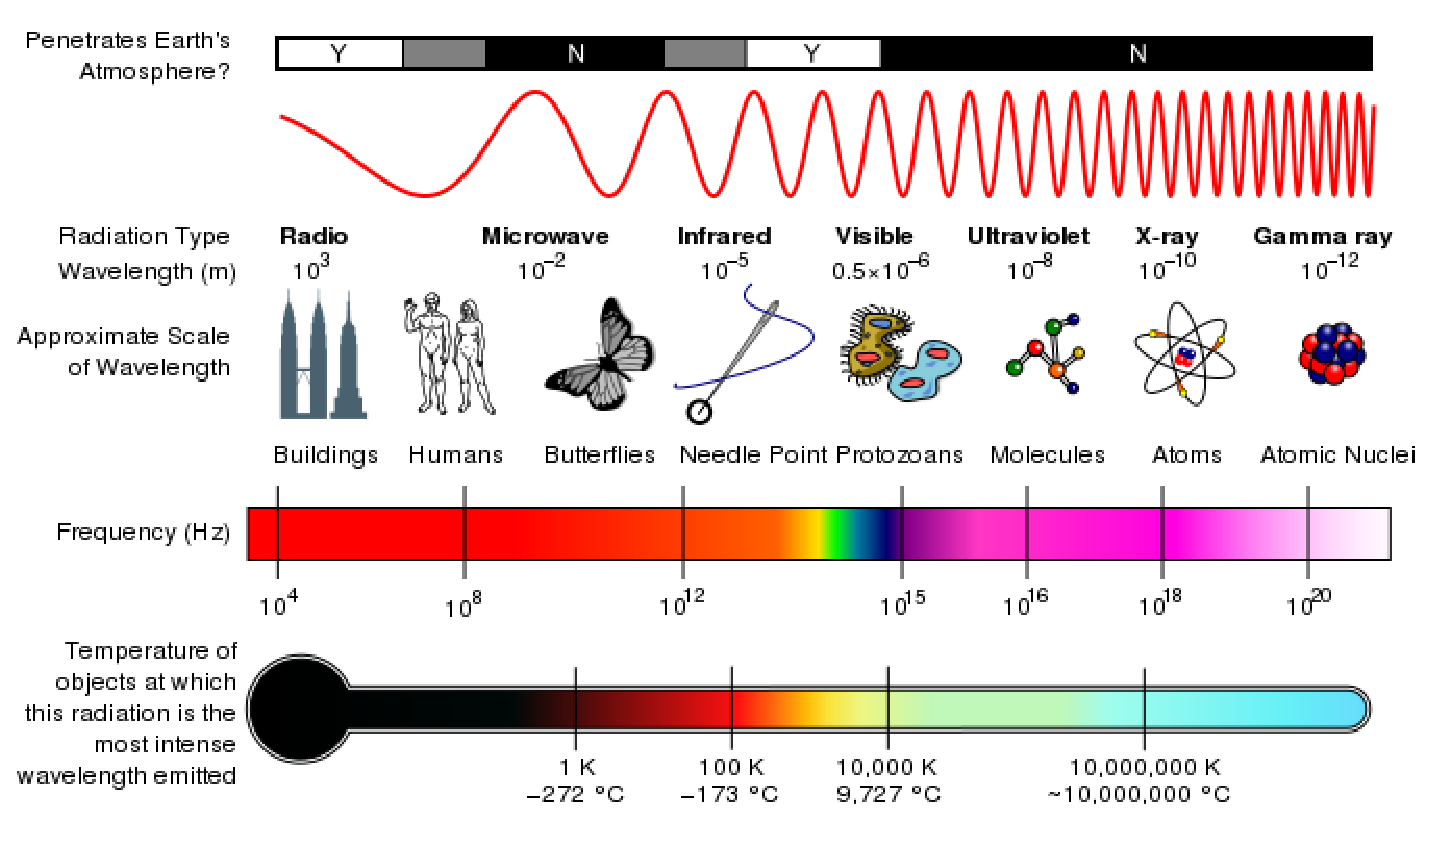
\includegraphics[width=0.95\textwidth]{../../epsimages/EM_Spectrum_Properties_edit.eps}%very big so leave out for now s}
\caption{The electromagnetic spectrum as a function of frequency. The different types according to wavelength are shown as well as everyday comparisons.}
\end{center}
\end{figure}

Observe the things around you, your friend sitting next to you, a large tree across the field. How is it that you are able to see these things? What is it that is leaving your friend's arm and entering your eye so that you can see his arm? It is light. The light originally comes from the sun, or possibly a light bulb or burning fire. In physics, light is given the more technical term electromagnetic radiation, which includes all forms of light, not just the form which you can see with your eyes. 

Electromagnetic radiation allows us to observe the world around us. It is this radiation which reflects off of the objects around you and into your eye. The radiation your eye is sensitive to is only a small fraction of the total radiation emitted in the physical universe. All of the different fractions taped together make up the electromagnetic spectrum. 

\Extension{Dispersion}{When white light is split into its component colours by a prism, you are looking at a portion of the electromagnetic spectrum.}

The wavelength of a particular electromagnetic radiation will depend on how it was created. 

\Exercise{Wave Nature of EM Radiation}{
\begin{enumerate}
\item List one source of electromagnetic waves. Hint: consider the spectrum diagram and look at the names we give to different wavelengths.
\item Explain how an EM wave propagates, with the aid of a diagram.
\item What is the speed of light? What symbol is used to refer to the speed of light? Does the speed of light change?
\item Do EM waves need a medium to travel through? 
\end{enumerate}
}

The radiation can take on any wavelength, which means that the spectrum is continuous. Physicists broke down this continuous band into sections. Each section is defined by how the radiation is created, not the wavelength of the radiation. But each category is continuous within the min and max wavelength of that category, meaning there are no wavelengths excluded within some range. 

The spectrum is in order of wavelength, with the shortest wavelength at one end and the longest wavelength at the other. The spectrum is then broken down into categories as detailed in Table~\ref{tab:emspectrum}.

\begin{table}[htbp]
\begin{center}
\caption{Electromagnetic spectrum}
\label{tab:emspectrum}
\begin{tabular}{|c|c|c|}\hline
\textbf{Category}&\textbf{Range of Wavelengths (nm)}&\textbf{Range of Frequencies (Hz)}\\\hline\hline
gamma rays&$<$1&$>3\times 10^{19}$ \\\hline
X-rays&1-10&$3\times 10^{17}$-$3\times 10^{19}$\\\hline
ultraviolet light&10-400&$7,5\times 10^{14}$-$3\times 10^{17}$\\\hline
visible light&400-700&$4,3\times 10^{14}$-$7,5\times 10^{14}$\\\hline
infrared&700-$10^{5}$&$3\times 10^{12}$-$4,3\times 10^{19}$\\\hline
microwave&$10^{5}-10^{8}$&$3\times 10^{9}$-$3\times 10^{12}$\\\hline
radio waves&$>10^{8}$&$<3\times 10^{9}$\\\hline
\end{tabular}
\end{center}
\end{table}


Since an electromagnetic wave is still a wave, the following equation that you learnt in Grade 10 still applies:
\nequ{c=f\cdot \lambda}


\begin{wex}{EM spectrum I}{Calculate the frequency of red light with a wavelength of $4,2 \times 10^{-7}$~m}{ 
We use the formula: $c=f\lambda$ to calculate frequency. The speed of light is a constant $3 \times 10^{8}$m/s.
\begin{eqnarray*}
c&=&f\lambda\\
3 \times 10^{8}&=&f \times 4,2 \times 10^{-7} \\
f &=& 7,14 \times 10^{14} \rm {Hz}
\end{eqnarray*}}
\end{wex}

\begin{wex}{EM spectrum II}
{Ultraviolet radiation has a wavelength of $200~\mathrm{nm}$. What is the frequency of the radiation?}
{\westep{To calculate the frequency we need to identify the
wavelength and the velocity of the radiation.}
Recall that all radiation travels at the speed of light ($c$) in vacuum.
Since the question does not specify through what type of material the Ultraviolet radiation
is traveling, one can assume that it is traveling through a vacuum.
We can identify two properties of the radiation - $wavelength
~(200~\mathrm{nm})$ and speed ($c$).
%From previous chapters, we know that the period of the wave
%is the time it takes
%for a wave to complete one cycle or one wavelength. 

\westep{We can use the equation $c = f \lambda$ to find the frequency since the wavelength is given.}
\begin{eqnarray*}
c &=& f \lambda \\
3 \times 10^{8} &=& f \times 200 \times 10^{-9} \\
f &=&  1.5 \times 10^{15} \ \rm{Hz}
\end{eqnarray*}
}
\end{wex}



Examples of some uses of electromagnetic waves are shown in Table~\ref{tab:emuses}. 

\begin{table}[htbp]
\begin{center}
\caption{Uses of EM waves}
\label{tab:emuses}
\begin{tabular}{|c|p{5cm}|}\hline
\textbf{Category}&\textbf{Uses}\\\hline\hline
gamma rays&used to kill the bacteria in marshmallows and to sterilise medical equipment\\\hline
X-rays&used to image bone structures\\\hline
ultraviolet light&bees can see into the ultraviolet because flowers stand out more clearly at this frequency\\\hline
visible light&used by humans to observe the world\\\hline
infrared&night vision, heat sensors, laser metal cutting\\\hline
microwave&microwave ovens, radar\\\hline
radio waves&radio, television broadcasts\\\hline
\end{tabular}
\end{center}
\end{table}

In theory the spectrum is infinite, although realistically we can only observe wavelengths from a few hundred kilometers to those of gamma rays due to experimental limitations. 

Humans experience electromagnetic waves differently depending on their wavelength. Our eyes are sensitive to visible light while our skin is sensitive to infrared, and many wavelengths we do not detect at all.

\Exercise{EM Radiation}
{
\begin{enumerate}
\item Arrange the following types of EM radiation in order of increasing frequency: infrared, X-rays, ultraviolet, visible, gamma. 
\item Calculate the frequency of an EM wave with a wavelength of 400~nm.
\item Give an example of the use of each type of EM radiation, i.e. gamma rays, X-rays, ultraviolet light, visible light, infrared, microwave and radio and TV waves.
\end{enumerate}
}

\section{The particle nature of electromagnetic radiation}
%\begin{syllabus}
%\item energy of a photon related to frequency and wavelength
%\item Calculate the energy of a photon using E = hf = hc/lambda
%\end{syllabus}

When we talk of electromagnetic radiation as a particle, we refer to photons, which are packets of energy. The energy of the photon is related to the wavelength of electromagnetic radiation according to:
%\equ{E=h\cdot f= \frac{hc}{\lambda}}{eq:ehf}
$h$ (called Planck's constant).






\Definition{Planck's constant}{Planck's constant is a physical constant named after Max Planck.

\nequ{h =6,626 \times 10^{-34}\ \mbox{J}\cdot\mbox{s}}
}

The energy of a photon can be calculated using the formula: $E=hf$ or $E=h \frac{c}{\lambda}$.
Where E is the energy of the photon in joules (J), h is planck's constant, c is the speed of light, f is the frequency in hertz (Hz) and $\lambda$ is the wavelength in metres (m).

\begin{wex}{Calculating the energy of a photon I}{Calculate the energy of a photon with a frequency of $3 \times 10^{18}$~Hz}
{
We use the formula: $E=hf$

\begin{eqnarray*}
E &=& hf\\
&=& 6,6 \times 10^{-34} \times 3 \times 10^{18}\\
&=& 2 \times 10^{-15} \eJ\\
\end{eqnarray*}}
\end{wex}

\begin{wex}{Calculating the energy of a photon II}
{What is the energy of an ultraviolet photon with a wavelength of 200~nm?}
{\westep{Determine what is required and how to approach the problem.}
We are required to calculate the energy associated with a photon of ultraviolet light with a wavelength of  200~nm.

We can use:
\nequ{E=h\frac{c}{\lambda}}

\westep{Solve the problem}
\begin{eqnarray*}
E & = & h\frac{c}{\lambda}\\
& = & (6,626 \times 10^{-34})\frac{3\times10^{8}}{200\times 10^{-9}}\\
& = & 9,939 \times 10^{-10}\eJ
\end{eqnarray*}}
\end{wex}


\subsection {Exercise - particle nature of EM waves}
\begin{enumerate}
\item How is the energy of a photon related to its frequency and wavelength?
\item Calculate the energy of a photon of EM radiation with a frequency of $10^{12}$~Hz.
\item Determine the energy of a photon of EM radiation with a wavelength of 600 nm.
\end{enumerate}

\section{Penetrating ability of electromagnetic radiation}
\label{p:em:emr12:pa}
%\begin{syllabus}
%\item Indicate the penetrating ability of the different kinds of EM radiation and relate it to energy of the radiation.
%\item Describe the dangers of gamma rays, X-rays and the damaging effect of ultra-violet radiation on skin
%\item Note: Link to Grade 11 Matter and Materials, atomic nuclei
%\end{syllabus}

Different kinds of electromagnetic radiation have different penetrabilities. For example, if we take the human body as the object. Infrared light is emitted by the human body. Visible light is reflected off the surface of the human body, ultra-violet light (from sunlight) damages the skin, but X-rays are able to penetrate the skin and bone and allow for pictures of the inside of the human body to be taken.

If we compare the energy of visible light to the energy of X-rays, we find that X-rays have a much higher energy. Usually, kinds of electromagnetic radiation with higher energy have higher penetrabilities than those with low energies.

Certain kinds of electromagnetic radiation such as ultra-violet radiation, X-rays and gamma rays are very dangerous. Radiation such as these are called ionising radiation. Ionising radiation transfers energy as it passes through matter, breaking molecular bonds and creating ions.
 
Excessive exposure to radiation, including sunlight, X-rays and all nuclear radiation, can cause destruction of biological tissue. 

\subsection{Ultraviolet(UV) radiation and the skin}
UVA and UVB are different ranges of frequencies for ultraviolet (UV) light. UVA and UVB can damage collagen fibres which results in the speeding up skin aging. In general, UVA is the least harmful, but it  can contribute to the aging of skin, DNA damage and possibly skin cancer. It penetrates deeply and does not cause sunburn. Because it does not cause reddening of the skin (erythema) it cannot be measured in the SPF testing. There is no good clinical measurement of the blocking of UVA radiation, but it is important that sunscreen block both UVA and UVB.

UVB light can cause skin cancer. The radiation excites DNA molecules in skin cells, resulting in possible mutations, which can cause cancer. This cancer connection is one reason for concern about ozone depletion and the ozone hole.

As a defense against UV radiation, the body tans when exposed to moderate (depending on skin type) levels of radiation by releasing the brown pigment melanin. This helps to block UV penetration and prevent damage to the vulnerable skin tissues deeper down. Suntan lotion, often referred to as sunblock or sunscreen, partly blocks UV and is widely available. Most of these products contain an SPF rating that describes the amount of protection given. This protection, however, applies only to UVB rays responsible for sunburn and not to UVA rays that penetrate more deeply into the skin and may also be responsible for causing cancer and wrinkles. Some sunscreen lotion now includes compounds such as titanium dioxide which helps protect against UVA rays. Other UVA blocking compounds found in sunscreen include zinc oxide and avobenzone.

\Extension{What makes a good sunscreen?}{
\begin{itemize}
\item UVB protection: Padimate O, Homosalate, Octisalate (octyl salicylate), Octinoxate (octyl methoxycinnamate)
\item UVA protection: Avobenzone
\item UVA/UVB protection: Octocrylene, titanium dioxide, zinc oxide, Mexoryl (ecamsule)
\end{itemize}

Another means to block UV is by wearing sun protective clothing. This is clothing that has a UPF rating that describes the protection given against both UVA and UVB.}

\subsection{Ultraviolet radiation and the eyes}
High intensities of UVB light are hazardous to the eyes, and exposure can cause welder's flash (photo keratitis or arc eye) and may lead to cataracts, pterygium and pinguecula formation.

Protective eyewear is beneficial to those who are working with or those who might be exposed to ultraviolet radiation, particularly short wave UV. Given that light may reach the eye from the sides, full coverage eye protection is usually warranted if there is an increased risk of exposure, as in high altitude mountaineering. Mountaineers are exposed to higher than ordinary levels of UV radiation, both because there is less atmospheric filtering and because of reflection from snow and ice.

Ordinary, untreated eyeglasses give some protection. Most plastic lenses give more protection than glass lenses. Some plastic lens materials, such as polycarbonate, block most UV. There are protective treatments available for eyeglass lenses that need it which will give better protection. But even a treatment that completely blocks UV will not protect the eye from light that arrives around the lens. To convince yourself of the potential dangers of stray UV light, cover your lenses with something opaque, like aluminum foil, stand next to a bright light, and consider how much light you see, despite the complete blockage of the lenses. Most contact lenses help to protect the retina by absorbing UV radiation.

\subsection{X-rays}
While x-rays are used significantly in medicine, prolonged exposure to X-rays can lead to cell damage and cancer.

For example, a mammogram is an x-ray of the human breast to detect breast cancer, but if a woman starts having regular mammograms when she is too young, her chances of getting breast cancer increases.

\subsection{Gamma-rays}
Due to the high energy of gamma-rays, they are able to cause serious damage when absorbed by living cells.

Gamma-rays are not stopped by the skin and can induce DNA alteration by interfering with the genetic material of the cell. DNA double-strand breaks are generally accepted to be the most biologically significant lesion by which ionising radiation causes cancer and hereditary disease.

A study done on Russian nuclear workers exposed to external whole-body gamma-radiation at high cumulative doses shows a link between radiation exposure and death from leukaemia, lung, liver, skeletal and other solid cancers.


\Extension{Cellphones and electromagnetic radiation}{Cellphone radiation and health concerns have been raised, especially following the enormous increase in the use of wireless mobile telephony throughout the world. This is because mobile phones use electromagnetic waves in the microwave range. These concerns have induced a large body of research. Concerns about effects on health have also been raised regarding other digital wireless systems, such as data communication networks.
In 2009 the World Health Organisation announced that they have found a link between brain cancer and cellphones.

Cellphone users are recommended to minimise radiation, by for example:

\begin{enumerate}
\item Use hands-free to decrease the radiation to the head.
\item Keep the mobile phone away from the body.
\item Do not telephone in a car without an external antenna.
\end{enumerate}

}

\subsection {Exercise - Penetrating ability of EM radiation}
\begin{enumerate}
\item Indicate the penetrating ability of the different kinds of EM radiation and relate it to energy of the radiation.
\item Describe the dangers of gamma rays, X-rays and the damaging effect of ultra-violet radiation on skin
\end{enumerate}
Presentation on the electromagnetic spectrum: SIYAVULA-PRESENTATION:http://cnx.org/content/m39513/latest/#slidesharefigure
\section {Summary}
\begin{enumerate}
\item Electromagnetic radiation has both a wave and a particle nature.
\item Electromagnetic waves travel at a speed of $3 \times 10^{8}~m \cdot s^{-1}$ in a vaccum.
\item The Electromagnetic spectrum consists of the follwing types of radiation: radio waves, microwaves, infrared, visible, ultraviolet, X-rays, gamma-rays.
\item Gamma-rays have the most energy and are the most penetrating, while radio waves have the lowest energy and are the least penetrating.

\end{enumerate}

\section{End of chapter exercise}
\begin{enumerate}

\item What is the energy of a photon of EM radiation with a frequency of $3 \times 10^{8}$~Hz? 

\item What is the energy of a photon of light with a wavelength of 660~nm?

\item List the main types of electromagnetic radiation in order of increasing wavelength.

\item List the main uses of:
\begin{enumerate}
\item radio waves
\item infrared
\item gamma rays
\item X-rays
\end{enumerate}

\item Explain why we need to protect ourselves from ultraviolet radiation from the Sun.

\item List some advantages and disadvantages of using X-rays.

\item What precautions should we take when using cell phones?

\item Write a short essay on a type of electromagnetic waves. You should look at uses, advantages and disadvantages of your chosen radiation.

\item Explain why some types of electromagnetic radiation are more penetrating than others.

\end{enumerate}


% CHILD SECTION END 



% CHILD SECTION START 

